\chapter{Results}
With the models established, we focus on their application.
First, the performance and general behavior of the \gls{BMB}, the Simulated Annealing and the Graphical LASSO will be compared on artificial data. 
In the subsequent section we apply the BMB and SA in context of HIV-1.
The SystemsX.ch HIV-X cohort \citep{HIVX} provides data of long-term patients whose viral reservoir were successfully suppressed with antiretroviral therapy.
Our main goal is to find possible interactions between the resistance relevant mutations gathered from the viral genotype and multiple clinical factors that quantify the success of the treatment.


\section{Application on Artificial Data}
We compare the Graphical LASSO, the Bayesian Markov Blanket and its Simulated Annealing variant on multiple artificial data sets, created as described in \autoref{subs:artdata}. 
In addition, we look at the behavior of the posterior distribution of $\Wxy$ experimentally for different values of $\lambda$.

In \autoref{fig:toy_example}, a small example for two synthetic data sets with $p=5$ and $q=15$ is shown.
Both the SA and the BMB were used for reconstructing the Markov Blanket of the $p$ query variables, with $lambda=70$ and $\lambda=1400$ respectively.
\begin{figure}[H]
	\centering
	\subfloat{
		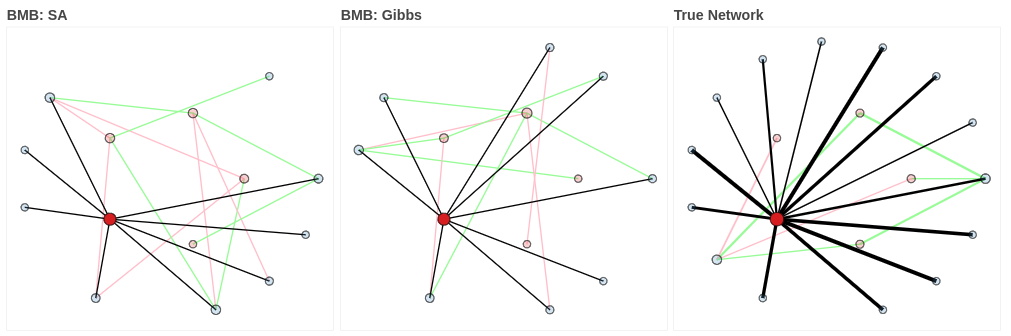
\includegraphics[width=1\linewidth]{network_ex_5_15}
	}
	\subfloat{
		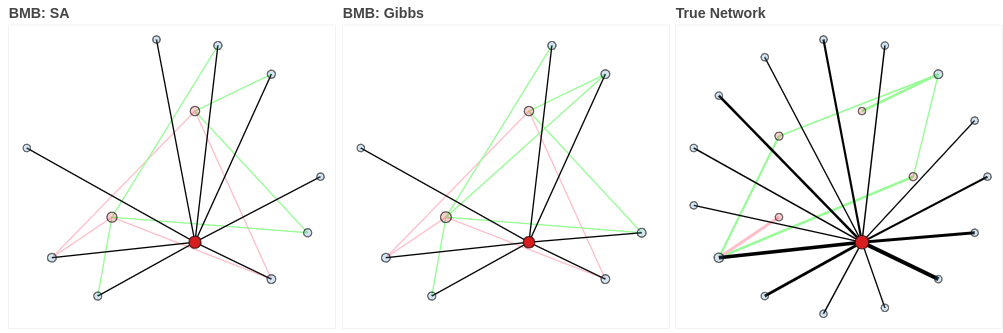
\includegraphics[width=1\linewidth]{network_ex_5_15_2}
	}
	\caption{Comparison of the true W12 subnetwork with the one resulting from the BMB ($lambda=70$) and SA ($\lambda=1400$) for two example networks with a threshold of $0.2$. The data was created similarly to the description in \autoref{subs:artdata}, but with $p=5$ and $q=15$.
		The red nodes correspond to the $p$ query variables.}
	
	\label{fig:toy_example}
\end{figure}
It can be seen that both networks are very similar, even though widely different $\lambda$ were used.
This is unexpected as the underlying model for both methods is the same.
In practice, finding an appropriate $\lambda$ is the most relevant part of the model selection,
as it is the only hyperparameter directly influencing the model.
Because of this, our focus in all three models will be the sparsity inducing hyperparameter and its effect on the quality of the reconstructed networks.

\subsection{Setup \& Model Hyperparameters}
Aim of the tests on the artificial data is a sound comparison between the original BMB and its Simulated Annealing variant.
As such, the methods should be set up in a similar way to avoid performance advantages simply due to parameter fine-tuning or the use of more computing resources (in our case iterations/sweeps) for either one.
The latter is especially important in the case of MCMC sampling and Simulated Annealing, where strong theoretical results for convergence exist.

We fix the number of total iterations in both samplers to 3000.
In the case of SA this refers to the summed amount of initial Gibbs sweeps, cooling steps and the draws from the cooled down system at temperature $T_n$.
As a consequence the computational effort is roughly equal between the two methods
\footnote{Only roughly, as the cooling part of the SA does not entail draws from the copula.}.
The detailed settings are shown in \autoref{table:settings_model}.
It should be noted that the burn-in is in both cases $0.3$ times the number of Gibbs Sweeps.

\begin{table}[H]
	\centering
	\caption{Model Parameters used for Testing\label{table:settings_model}}
	\begin{tabular}{l c c}
		& \textbf{BMB}   & \textbf{Simulated Annealing} \\
		\toprule
		Total Iterations  & $3000$         & $3000$                       \\\midrule
		Gibbs Sweeps      & $3000$         & $900$                        \\
		Burn-In           & $900$          & $270$                        \\
		Credible Interval & $[0.15, 0.85]$ & $[0.15, 0.85]$               \\
		Cooling Steps     & -              & $2100$                       \\
		Draws at $T_n$    & -              & $300$                        \\
		$T_0$             & -              & $1$                          \\
		$T_n$             & -              & $0.01$                       
	\end{tabular}
\end{table}

With these settings, the models were applied to 40 artificially created data sets with $p=10$ and $q=90$.

\subsection{Restrictions on Lambda}
\autoref{fig:sparsitybylambda} displays the average fraction of zero-edges (i.e. a measure of sparsity) of the reconstructed networks in relation to the chosen $\lambda$.
\begin{figure}
	\centering
	\subfloat{
		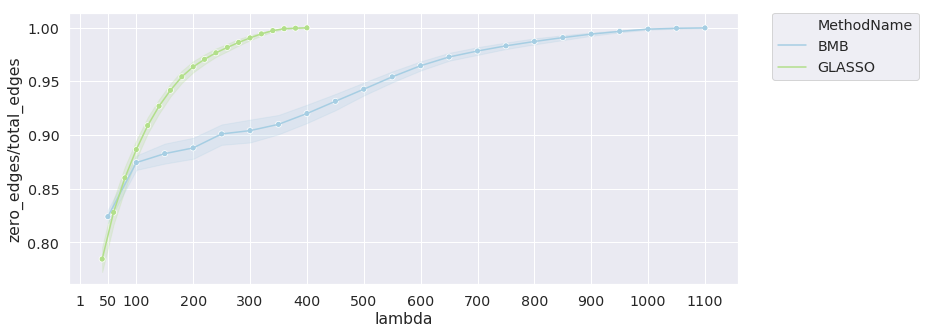
\includegraphics[width=0.9\linewidth]{sparsity_bylambda_GLBMB}
	}
	\subfloat{
		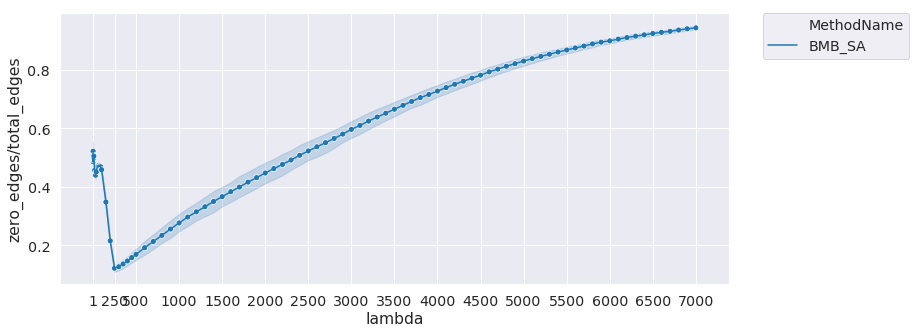
\includegraphics[width=0.9\textwidth]{sparsity_bylambda_SA}
	}
	
	\caption{Sparsity of Networks for different $\lambda$ over all 40 data sets.
		Plotted points correspond to the mean over all datasets and error bars to a $95\%$ bootstrapping confidence interval for the mean.}
	\label{fig:sparsitybylambda}
\end{figure}
The $\lambda$ were restricted to ranges that result in non-trivial (i.e. not empty) graphs. 
Furthermore, computational issues cause a lower bound for the GLASSO and an upper bound for the SA.
Lambdas below $100$ led to convergence problems for the Graphical LASSO, even in the case of a high number ($50000$) of iterations.
Conversely, SA has an upper bound due to numerical instability.
With increasingly high $\lambda$ the MGIG draws of the $\Wxx$ block (see \autoref{sample_MGIG}) and more specifically the inversion
$$
A=(\Wxy(\matr{S}_{22}+\matr{I})\Wxy^T)^{-1}
$$
fails as $A^{-1}$ becomes nearly singular.
We suspect the continued fraction of Wisharts to be a major cause of numerical instability in the sampler.
Decreasing the number of fractions used for sampling the MGIG increases the maximum possible $\lambda$ before failure, supporting this assumption.
While all three methods generally follow the trend of getting sparser for higher $\lambda$, the scale on which this happens is vastly different. 
Especially the Simulated Annealing requires a much higher $\lambda$ for the same level of sparsity as the BMB and GLASSO.
Aside from that, the BMB and SA behave differently than expected for very low $\lambda$.
Both recreate denser networks again, with the effect being more pronounced in the Annealing.
A problem possibly underlying this can be identified by comparing the MCMC diagnostic plots for the different $\lambda$.
\autoref{fig:diag_SA_l7000} shows the MCMC diagnostics for SA with a $\lambda$ of 7000.
\begin{figure}[H]
	\centering
	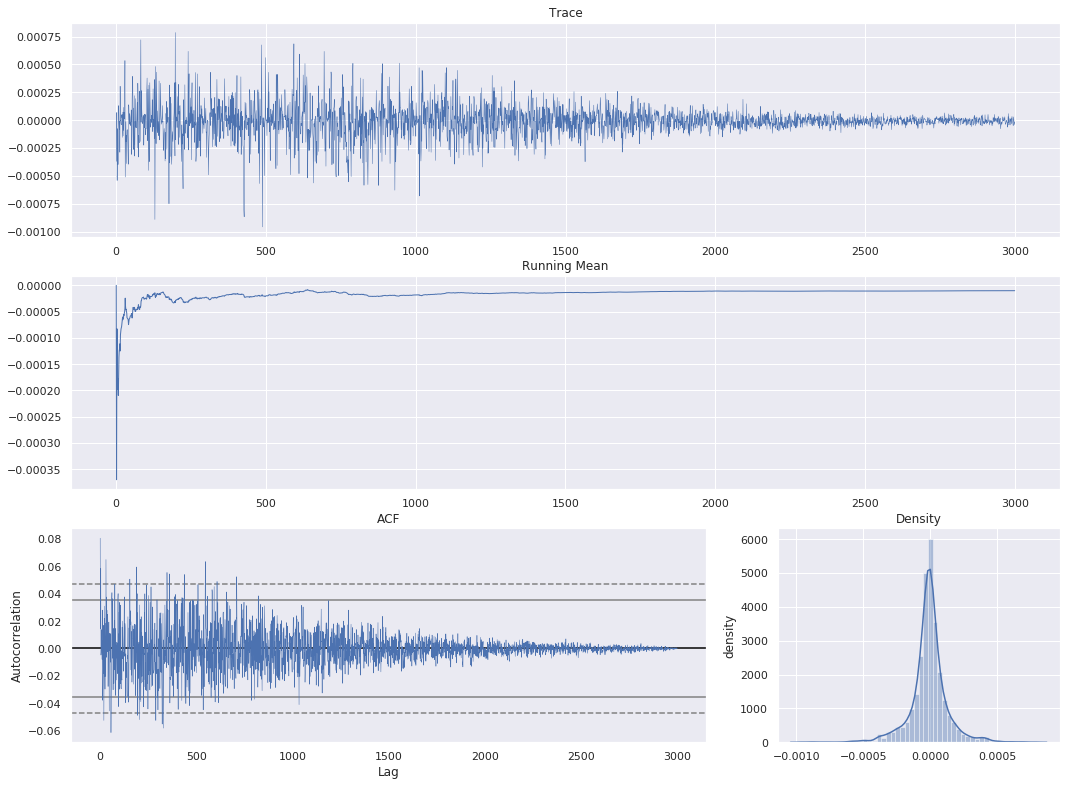
\includegraphics[width=0.7\textwidth]{diag_SA_l7000}
	\caption{MCMC Diagnostics: Simulated Annealing with a $\lambda$ of 7000}
	for the posterior marginal $(\Wxy)_{14}$.
	\label{fig:diag_SA_l7000}
\end{figure}
In the trace plot we can clearly see the effect of the Annealing.
Starting at iteration 1000, the system cools down and the samples slowly focus more on the region around the MAP.
Furthermore, the density plot indicates the marginal being unimodal%
\footnote{Note that the density plots of the Annealing includes \textit{all} drawn samples and only serves an diagnostic purpose.
	The actual estimation is only based on samples drawn at the target temperature.}.
When switching to a low $\lambda$ (see \autoref{fig:diag_SA_l20}), the cooled down chain starts fluctuating between two points,
which is also reflected in the very high autocorrelation switching signs for each lag.
As Simulated Annealing eventually samples from all global maxima, this behavior as well as the density plot indicates a multi-modality in the posterior marginals.
This effect gets more pronounced for smaller $\lambda$ as shown in \autoref{fig:diag_SA_l20},
where the distance between the modes also increases.
Since the modes seemingly diverge further from each other for lower $\lambda$, the Credible Interval also increases and is more likely to cover the origin, estimating an edge as 0.
This might explain the sparser networks for very small $\lambda$.

\begin{figure}
	\centering
	\subfloat{
		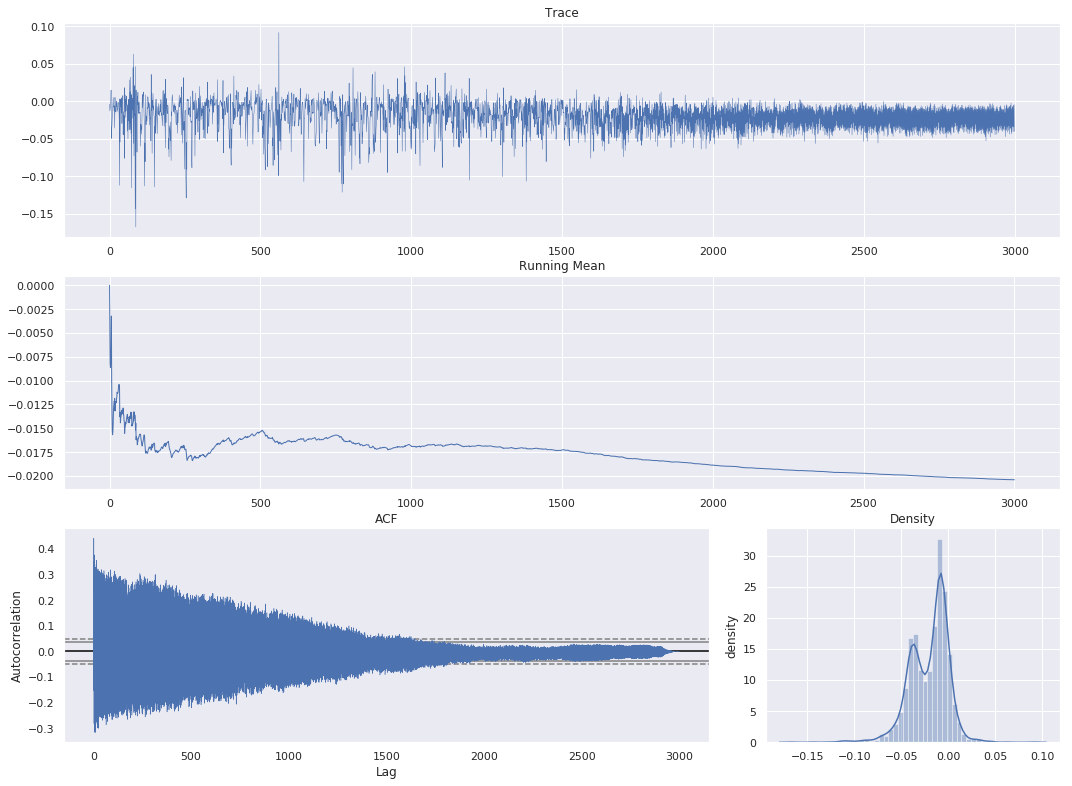
\includegraphics[width=0.8\linewidth]{diag_SA_l90}
	}
	\subfloat{
		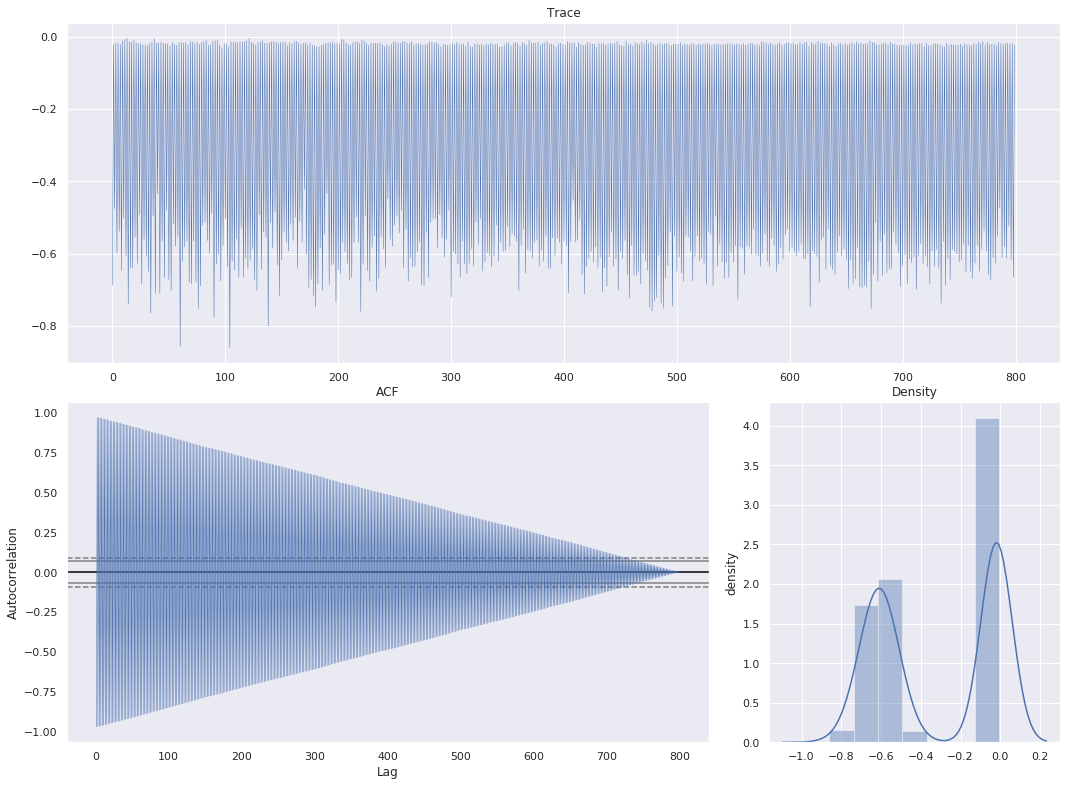
\includegraphics[width=0.8\textwidth]{diag_SA_l20}
	}
	\caption{MCMC Diagnostics: Simulated Annealing with a $\lambda$ of 90 (top) and 20 (bottom) }
	for the posterior marginal $(\Wxy)_{14}$.
	\label{fig:diag_SA_l20}
\end{figure}
In case of the standard BMB this behavior appears more subtle, but is still existent and can be observed for extremely small $\lambda$ (see \autoref{fig:diag_GIBBS_l1_400}).
But in this case, a high autocorrelation and jumping between values indicate mixture problems of the Markov chain. A possible cause might be numerical problems for low $\lambda$.
The hyperparameter $\lambda$ indirectly affects the diagonal of $\matr{C}$, which has to be inverted for draws of the $\Wxy$ block (see \autoref{W12_draw}).
However, the Markov chains corresponding to $\lambda$ in the range of $200$ to $300$ (where the bimodality in the SA marginals begins) did not exhibit similar problems, and neither could we observe any bimodal behavior in the non-cooled marginals.
%TODO

So the question arises whether multi-modality in the posterior actually exists for low $\lambda$ ($<300$) or just occurs as a side-effect of the Markov chains convergence problems.
In the next section we will expand on this by looking the empirical posteriors of $\Wxy$ for relatively small $\lambda$ that do not exhibit unusual behavior of the Markov chain.

Regardless of the outcome, it can already be seen that the $\lambda$s below $300$ do not lead to reasonable estimates 
for SA with the current thresholding method based on Credible Intervals.
Because of this, they will be disregarded for the performance evaluation in \autoref{ss:quality}.
Furthermore, $\lambda$ below $50$ will be ignored for the Gibbs BMB due to convergence problems.

\begin{figure}
	\centering
	\subfloat{
		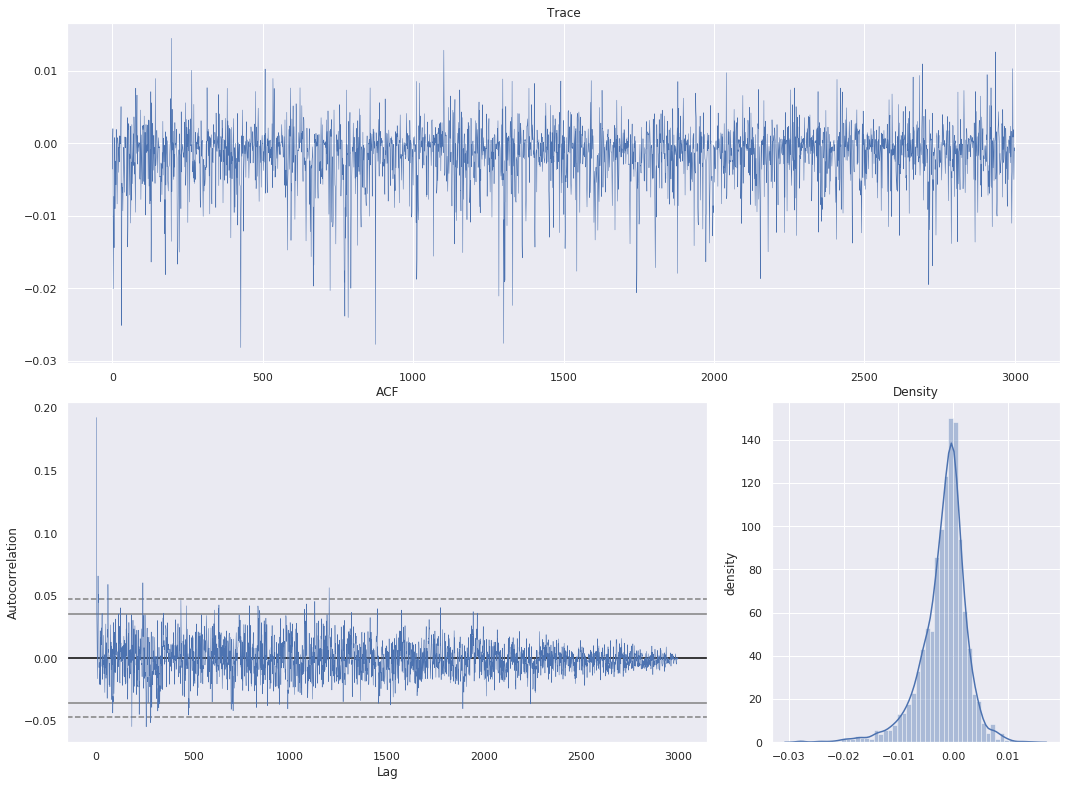
\includegraphics[width=0.8\linewidth]{diag_GIBBS_l400}
	}
	\subfloat{
		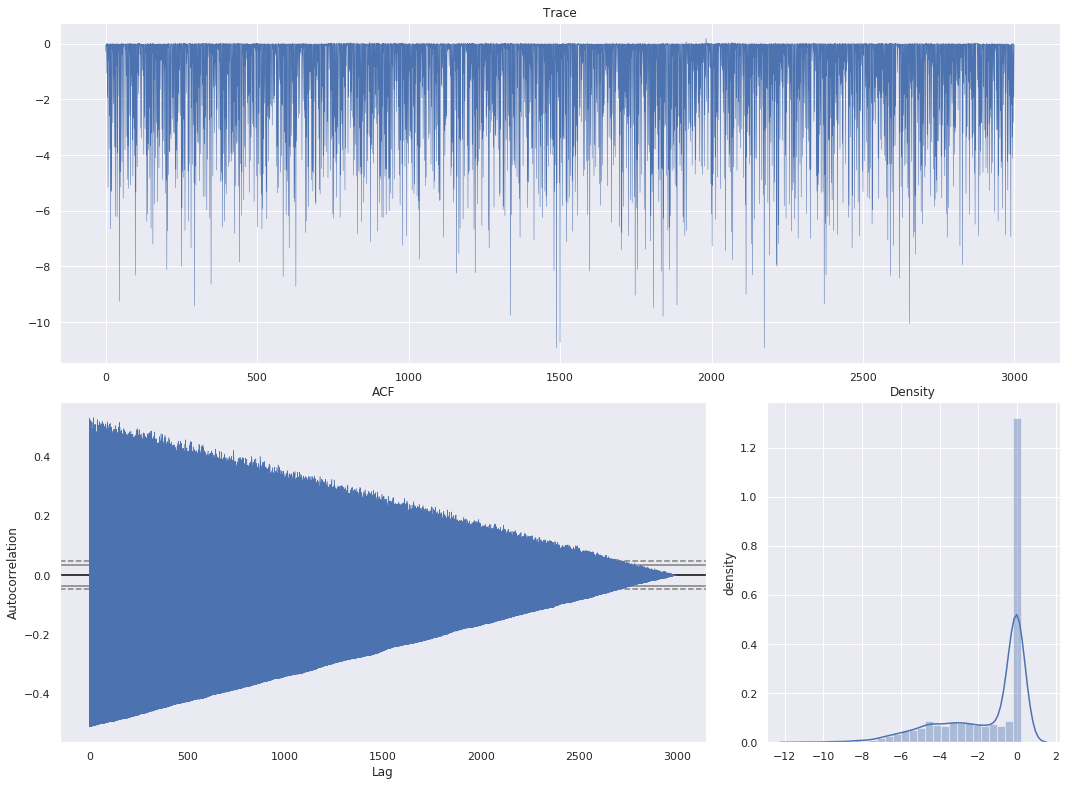
\includegraphics[width=0.8\textwidth]{diag_GIBBS_l1}
	}
	
	\caption{MCMC Diagnostics: BMB with a $\lambda$ of 400 (top) and 1 (bottom)}
	for the posterior marginal $(\Wxy)_{14}$.
	\label{fig:diag_GIBBS_l1_400}
\end{figure}

\FloatBarrier
\subsection{Modality of the Posterior}
\label{ss:modality}
In Chapter 3 we already mentioned that the modality of the posterior is important to consider when choosing an estimation method.
Additionally, the results of the previous section indicated that the posterior marginals of the individual $\Wxy$ edges get bimodal for very low $\lambda$. 
Instead of individual edges, we now look at the marginal posterior $ p(\Wxy|\matr{S}, \lambda)$ \footnote{$p(\Wxy | \matr{S}, \lambda)$ has shown to behave similarly to $p(\Wxy | \hat{S}, \lambda)$ for the Gibbs sampler, presumably because the copula does not have a big influence on Gaussian test data.}.
For this, linear \gls{PCA} was applied to reduce the dimensionality of the posterior.
The empirical distribution can then be observed alongside the first principal components.

In \autoref{fig:unimodality_art300}
the empirical posterior marginal of $\Wxy$ for one artificial data set is shown alongside the first principal components for $\lambda=300$.
%%%%%%%%%%%%%%% one mode artificial data
\begin{figure}[H]
	\centering
	\subfloat{
		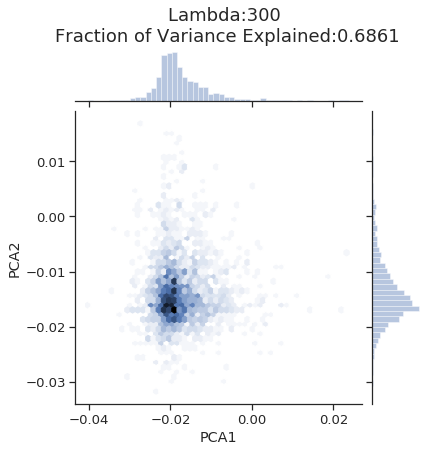
\includegraphics[width=0.48\linewidth]{PCA_W12_art_l300}
	}
	\subfloat{
		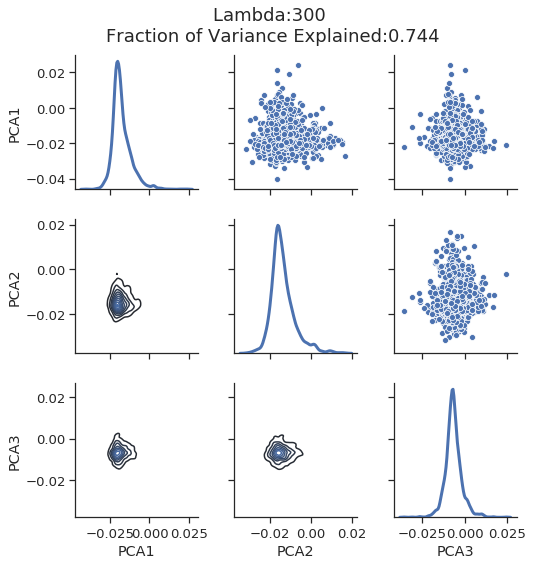
\includegraphics[width=0.48\linewidth]{PCA_W12_art_l300_2}
	}
	\caption{Empirical distribution of the $\Wxy$ posterior marginal over the first principal components for one example data set with $\lambda=300$.}
	
	\label{fig:unimodality_art300}
\end{figure}
It can be seen that the posterior is unimodal with a lot of mass surrounding the mode.
In contrast, a slightly lower $\lambda$ of $200$ already gets bimodal, as shown in \autoref{fig:unimodality_art200}.
%%%%%%%%%%%%%% multiple modes artificial data
\begin{figure}[H]
	\centering
	\subfloat{
		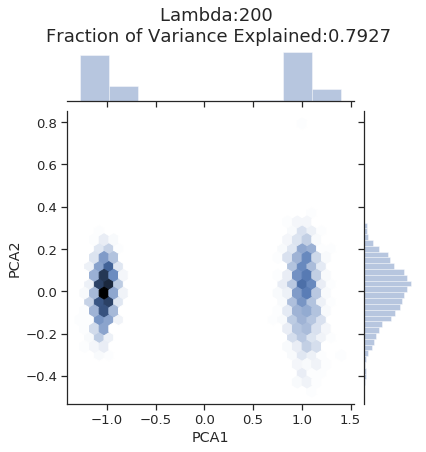
\includegraphics[width=0.48\linewidth]{PCA_W12_art_l200}
	}
	\subfloat{
		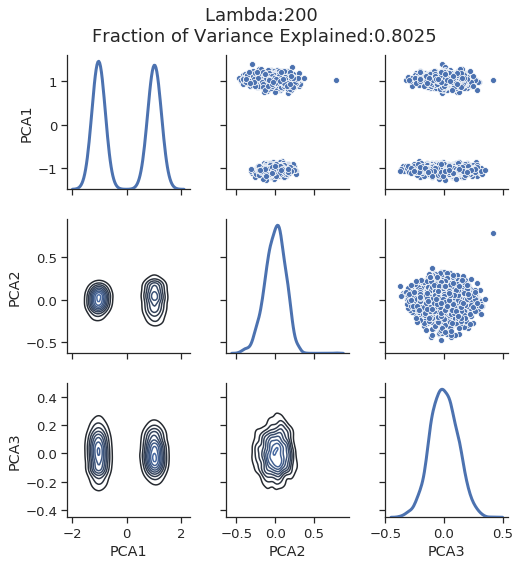
\includegraphics[width=0.48\linewidth]{PCA_W12_art_l200_2}
	}
	\caption{Empirical distribution of the $\Wxy$ posterior marginal over the first principal components for one example data set with $\lambda=200$.}
	
	\label{fig:unimodality_art200}
\end{figure}
Additionally, the distribution seems flatter alongside the first principal component. 
The corresponding MCMC diagnostics do not indicate any issues with the convergence in this range of $\lambda$.
%TODO show MCMC diag of lambda 200
As far as can be ascertained, the posterior stays unimodal for higher $\lambda$ and multi-modal for lower ones.
This change of modality aligns to the sudden change of sparsity of the Annealing in \autoref{fig:sparsitybylambda},
confirming that the fluctuation is indeed between two modes and not a result of numerical instability or bad mixing of the chain.
Consequently we can assume that the posterior distribution of $\Wxy$ actually is multi-modal for low $\lambda$.

An other interesting observation is that the variance explained by the first few principal components decreases for higher $\lambda$.
This could be due to the regularizing effect of the $\lambda$.
Aside from enforcing sparsity, the prior also decreases the values of the non-zero edges significantly.
If variance in the non-zero edges decreases faster than the variance of the zero-edges  (in terms of absolute values), the variance in the distribution is not anymore dominated by the non-zero edges.
This is illustrated in \autoref{fig:pca123}, where the distribution of a (truly) non-zero edge is compared to a zero edge
for a specific data set. 
Initially, the variance of the non-zero dominates and the PCA would still be able to a lot of information with just one axis. For higher $\lambda$ however, this changes and the joint distribution becomes more circular,
leaving a linear PCA no possibility to summarize the data in a low-dimensional projection (in this case onto one axis).
For higher dimensional data the behavior should be similar, with the joint distribution tending towards a sphere.

\begin{figure}
	\centering
	\subfloat{
		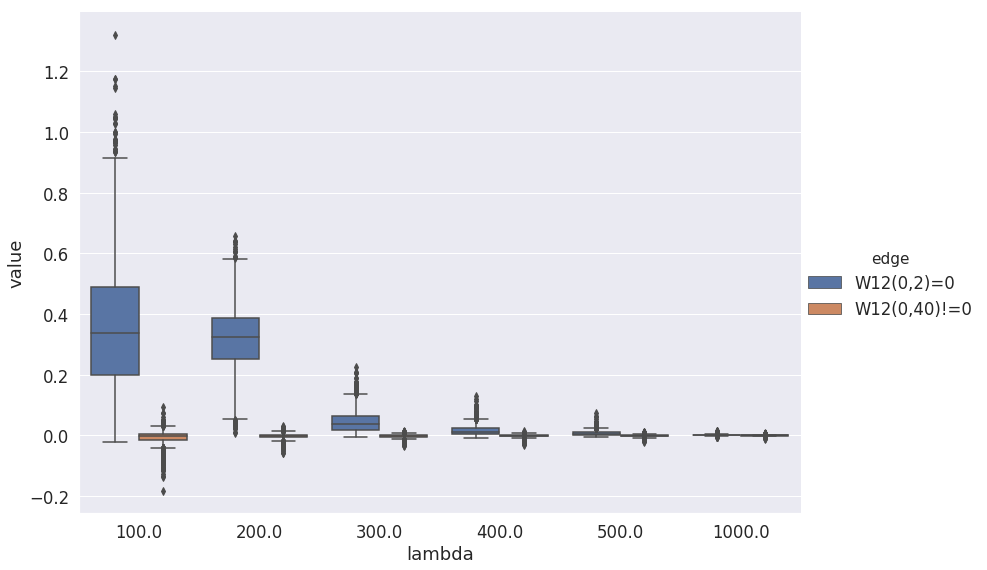
\includegraphics[width=0.8\textwidth]{pca_boxplot}
	}
	\qquad\qquad\qquad\qquad\qquad\qquad\qquad\qquad\qquad \\
	\subfloat{
		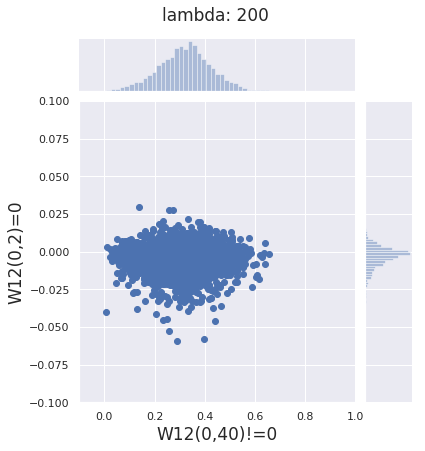
\includegraphics[width=0.31\textwidth]{pca1}
	}
	\subfloat{
		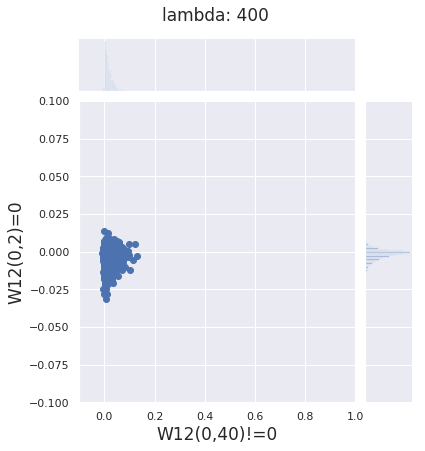
\includegraphics[width=0.31\textwidth]{pca2}
	}
	\subfloat{
		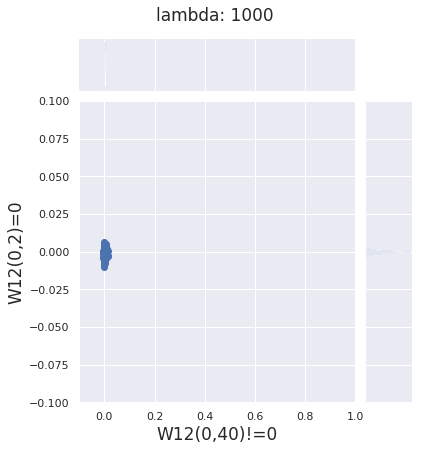
\includegraphics[width=0.31\textwidth]{pca3}
	}
	\caption{The effect of a higher $\lambda$ on the joint distribution between two marginals of the $\Wxy$ block. The true edge of $(\Wxy)_{(0,40)}$ (x-axis) is non-zero, while the true edge of $(\Wxy)_{(0,2)}$ (y-axis) is zero.}
	\label{fig:pca123}
\end{figure}


We now know the modality of $p(\Wxy | \lambda)$, but Simulated Annealing estimates the MAP of the joint posterior $p(\Wxx, \Wxy, \matr{T} | \hat{S}, \lambda)$.
Unfortunately we are unable infer anything significant about the joint posterior because the first few (2-3) principal components only explain a low amount of the variance ($<10\%"$), rendering the 2 dimensional projection useless.





\subsection{Quality of Reconstructed Networks}
\label{ss:quality}
With the range of possible $\lambda$ established, the predictive performance of the individual methods can be analyzed.

The performance metrics for the \gls{BMB}, GLASSO and \gls{SA} are visualized in \autoref{fig:metrics_BMB}.
We plotted the mean over all datasets as well as error bars corresponding to a $95\%$ bootstrapping confidence interval for the mean.
\begin{figure}
	\centering
	\subfloat{
		\makebox[\textwidth][c]{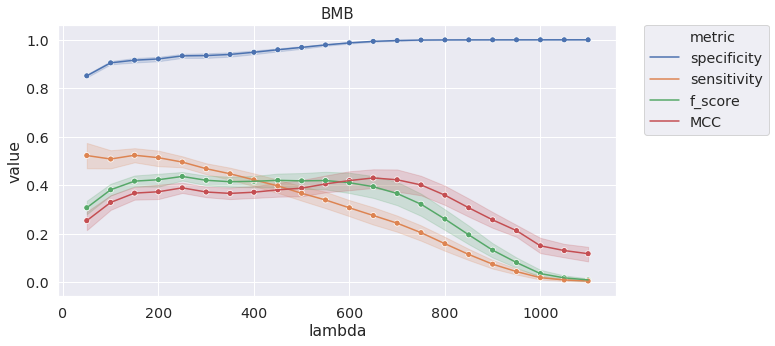
\includegraphics[width=1.05\textwidth]{metrics_BMB}}%
	}
	\subfloat{
		\makebox[\textwidth][c]{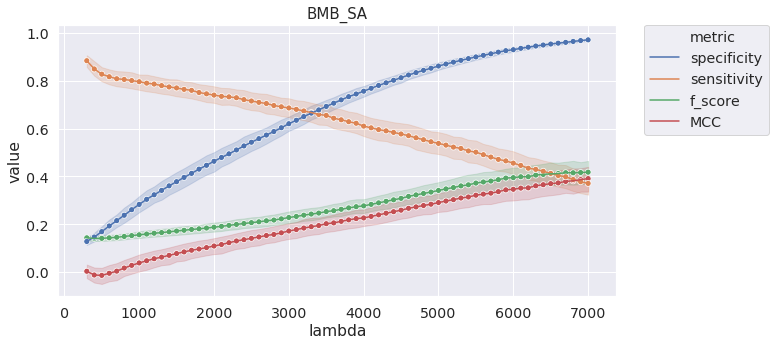
\includegraphics[width=1.05\textwidth]{metrics_SA}}%
	}
	\subfloat{
		\makebox[\textwidth][c]{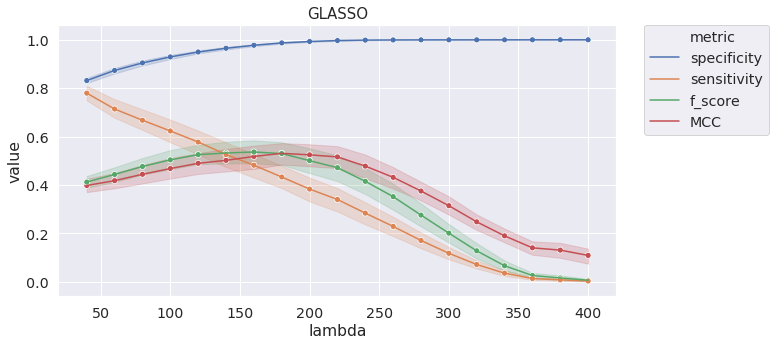
\includegraphics[width=1.05\textwidth]{metrics_GLASSO}}%
	}
	\caption{Average performance metrics for the Gibbs BMB, Simulated Annealing, and the GLASSO.
		The shaded area corresponds to a 95\% bootstrapping confidence interval for the mean.}
	\label{fig:metrics_BMB}
\end{figure}
First of all, the effect of the $\lambda$ on the specificity is of interest.
It can be seen that the specificity generally increases with a higher $\lambda$ for all three methods, which is to be expected due to its sparsity inducing property.
Furthermore, there is a linear relationship between the fraction of nonzero edges and the specificity, as shown in \autoref{fig:sparsity_vs_specificity}.
In practical applications we can only observe the resulting network, so this relation is very useful.
We can effectively control for the specificity by adjusting $\lambda$ until a satisfactory density of the network graph is reached.
\begin{figure}
	\centering
	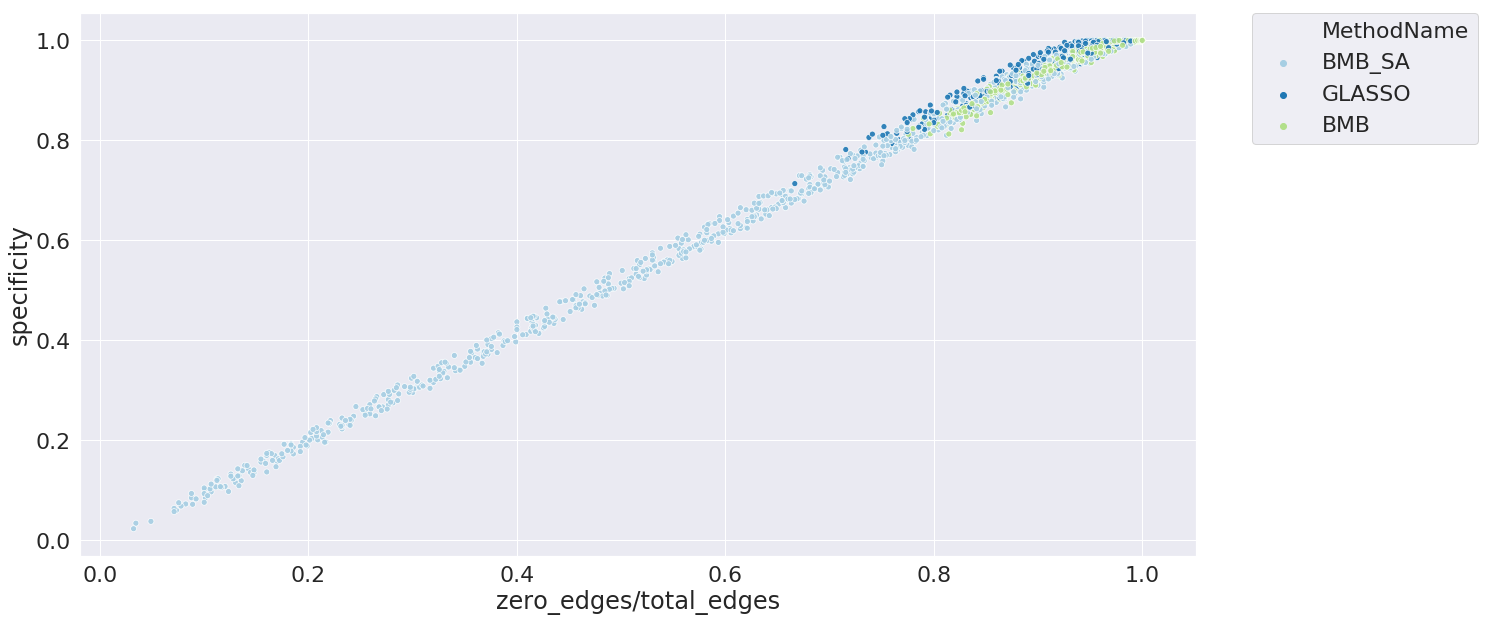
\includegraphics[width=0.9\textwidth]{sparsity_vs_specificity}
	\caption{Relation between the sparsity in the reconstructed networks and the resulting specificity for all 40 data sets.}
	\label{fig:sparsity_vs_specificity}
\end{figure}
While the BMB and GLASSO show a maximum average MCC and F-score at around 600 and 200 respectively, the limited range of the Annealing seems to not include it's maximum.
But the drop in sensitivity for very high $\lambda$ will also have to occur in the Annealing as the networks will presumably be empty for a high enough $\lambda$.
With the specificity already getting close to 1, we can thus assume that we would not observe much of an improvement for slightly higher $\lambda$.
Nonetheless, the Annealing reaches values of around 0.4 for both the F-Score and the MCC, which are comparable to the performance of the BMB.
But in all cases, the SA and BMB are outperformed by the GLASSO.
Aside from that, the Annealing is capable of covering a wider range of the sensitivity, allowing the estimation of less sparse networks.

To show the similarity between the methods, we fix $\lambda$ such that the resulting network size for the test data is (close to) equal in all methods.
In \autoref{fig:boxplot_metrics_fixlambda}  the performance for individual data sets is shown for these fixed $\lambda$. 
While the GLASSO always has the highest MCC and F-score, the difference between the Annealing and the BMB is not that well-defined.
In addition, the methods mostly agree on the relative performance for the specific data sets.
For example, all show low performance on data sets 160 and 180 while performing well on 178.
%%%%%%%%% for each dataset with fixed lambda
\begin{figure}
	\centering
	\subfloat{
		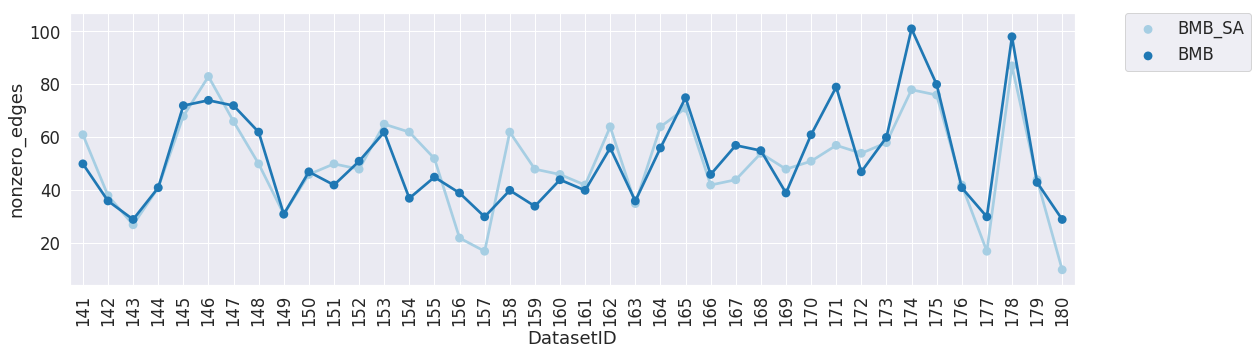
\includegraphics[width=\linewidth]{fixlambda_sparsity}
	}
	\subfloat{
		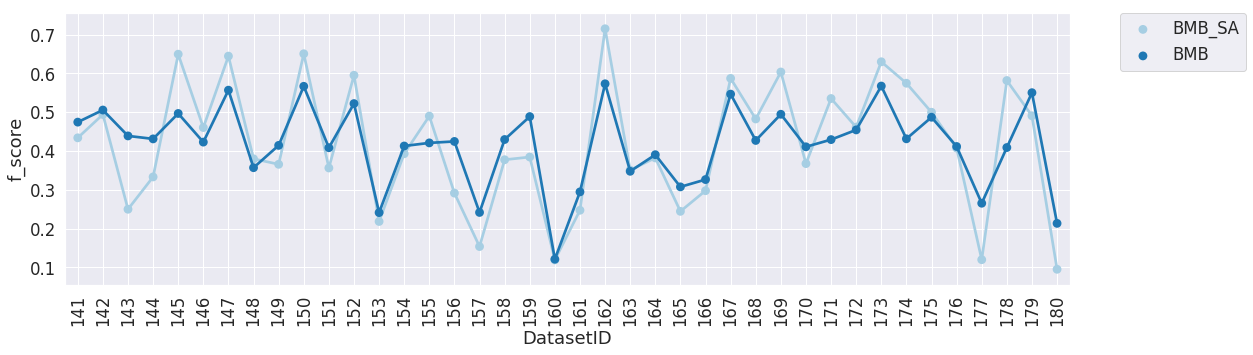
\includegraphics[width=\linewidth]{fixlambda_fscore}
	}
	\subfloat{
		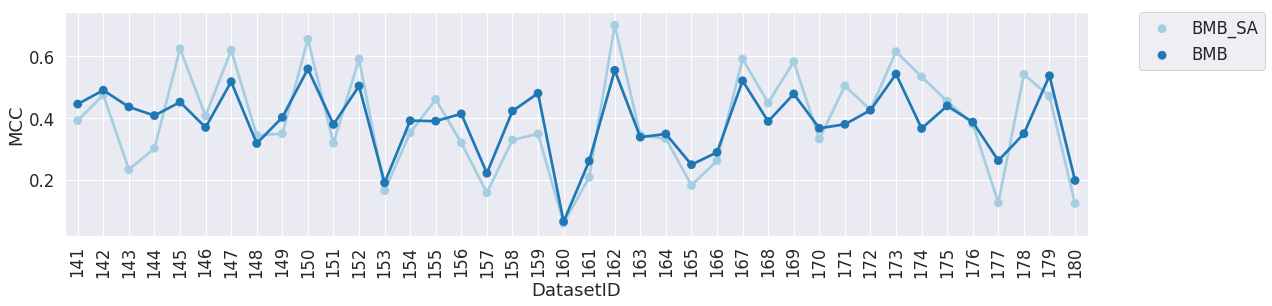
\includegraphics[width=\linewidth]{fixlambda_MCC}
	}
	\caption{Different Metrics for fixed $\lambda$ resulting in a roughly similar network size.}
	\label{fig:fix_lambda_bydataset}
	$\lambda_{BMB}=500 \quad$
	$\lambda_{SA}=7000\quad$
	$\lambda_{GLASSO}=150$
\end{figure}
Aside from confirming the previous results, the box-plots in \autoref{fig:fix_lambda_bydataset} furthermore show that the Annealing exhibits a higher variance among different data sets than the BMB for basically all metrics, excluding the specificity (with fixed $\lambda$).

%%%%%%%%%%%%%%%% boxplots fixed lambda
\begin{figure}
	\centering
	\subfloat{
		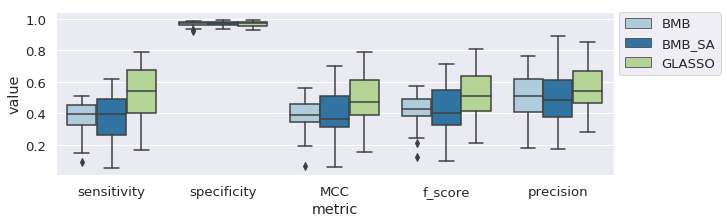
\includegraphics[width=0.9\linewidth]{boxplot_metrics_fixlambda}
	}
	\subfloat{
		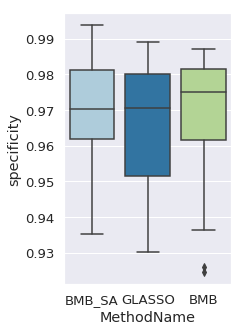
\includegraphics[width=0.25\linewidth]{boxplot_metrics_fixlambda_spec}
	}
	\caption{Different Metrics for fixed $\lambda$ resulting in an approximately similar network size.}
	\label{fig:boxplot_metrics_fixlambda}
	$\lambda_{BMB}=500 \quad$
	$\lambda_{SA}=7000\quad$
	$\lambda_{GLASSO}=150$
\end{figure}

Finally, we will look at how the performance of the methods relate to the sparsity for easing the search of a suitable $\lambda$ in practice.
While information criteria such as the (extended) BIC \citep{foygel2010extended} are popular for model selection of \gls{GGM}s, they are based on the calculation of the (log) likelihood, which requires the complete matrix $\W$.
In our current setting for the Simulated Annealing,
the whole precision matrix is not available since cooling the $\Wyys$ block would change the estimated joint MAP (see \autoref{ss:joint_map}).
Consequently we have to look at networks resulting from a range of different $\lambda$ and see how they change for different $\lambda$.
In this case, knowing how the model generally behaves in relation to the sparsity can then be helpful.
\autoref{fig:hexbin} shows the relation between the number of zero-edges and the metrics.
We can see that both the F-Score and the MCC are highest when in the range corresponding to the true sparsity of the networks (which is between around $90\%$ to $94.\overline{4}\%$).
After reaching this point, the sensitivity drops sharply for sparser graphs while the specificity only increases slowly,
thus resulting in a decrease of the F-score and MCC.
However, even for higher sparsity the specificity does not always reach $100\%$ for non-trivial graphs.
So for avoiding false positives it is advisable to overestimate the sparsity of the target network when selecting a $\lambda$.
Aside from that, the plots agree with the previous results in relation to the $\lambda$.

%%%%%%%%%%%%%%% sparsity vs others, hexbin with polynomial regression
\begin{figure}
	\centering
	\subfloat{
		\makebox[\textwidth][c]{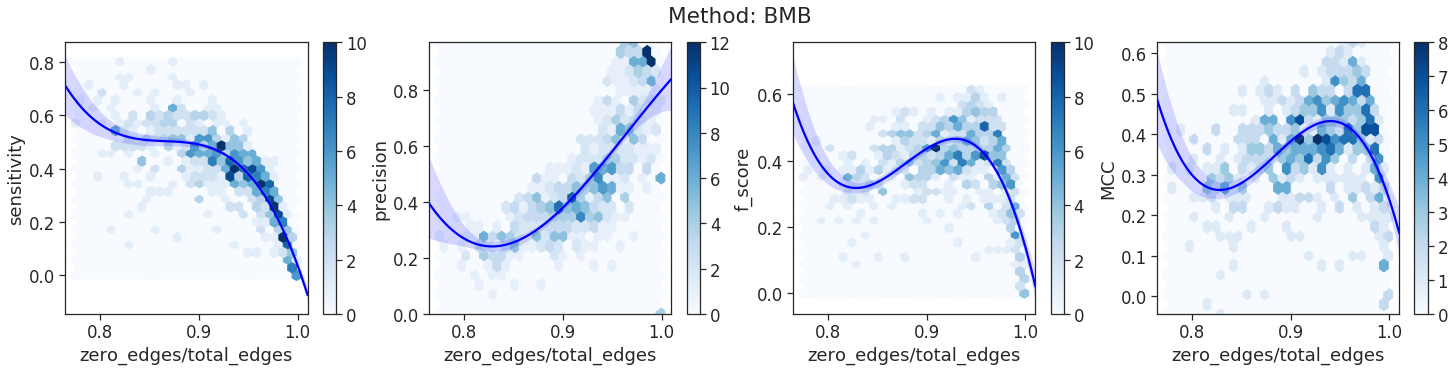
\includegraphics[width=1.2\textwidth]{sparsity_vs_all_BMB}}%
	}
	\subfloat{
		\makebox[\textwidth][c]{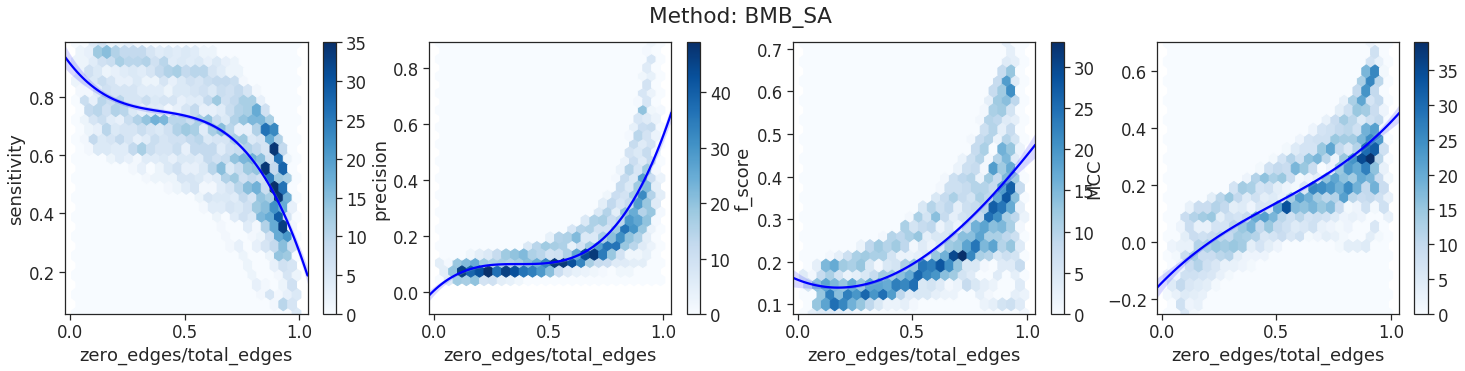
\includegraphics[width=1.2\textwidth]{sparsity_vs_all_BMB_SA}}%
	}
	\subfloat{
		\makebox[\textwidth][c]{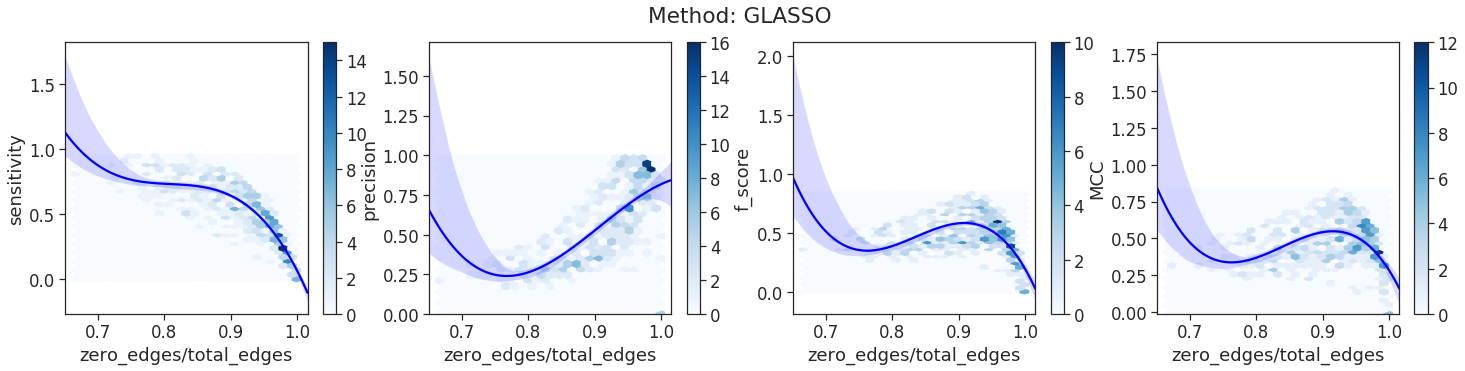
\includegraphics[width=1.2\textwidth]{sparsity_vs_all_GLASSO}}%
	}
	\caption{Relationship between the sparsity of the reconstructed Network and different performance measurements.
		The plots were created using 2D histograms with hexagon binning and a polynomial regression of degree 3.}
	\label{fig:hexbin}
\end{figure}
\FloatBarrier

The similarity of the resulting networks for the BMB and SA is illustrated in \autoref{fig:graph_BMB_MCC} and \autoref{fig:graph_SA_MCC}.
While they still slightly differ, we could not find any consistent advantage in either of them (in terms of the used measures).
More sophisticated graph comparison methods would be necessary for a better understanding of their actual differences.
Attempts at combining the two methods by intersection of the resulting graphs has proven to be difficult due to the different scales of $\lambda$.
Even when parameters resulting in the same network size were found, the combinations did not provide any significant improvement.
\begin{figure}
	\centering
	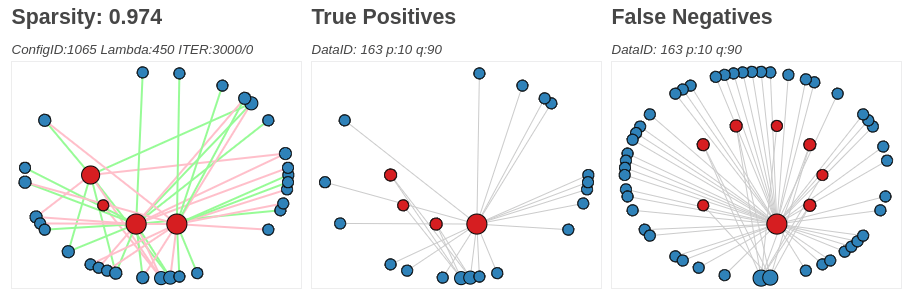
\includegraphics[width=1\linewidth]{graph_BMB_0974}
	\caption{W12 subnetwork reconstructed with Gibbs BMB (for artificial data with id 162)}
	\label{fig:graph_BMB_MCC}
\end{figure}
\begin{figure}
	\centering
	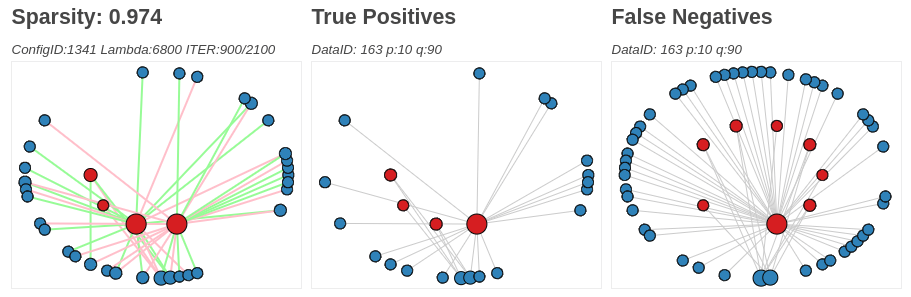
\includegraphics[width=1\linewidth]{graph_SA_0974}
	\caption{W12 subnetwork reconstructed with SA (for artificial data with id 162)}
	\label{fig:graph_SA_MCC}
\end{figure}


\FloatBarrier
\section{Application on Real Data: HIV-X}
We now switch to the Markov Blanket estimation in context of the HIV-X MRD Project \citep{HIVX}.

The \gls{HIV} is one of the most widespread and harmful viruses in the world.
If left untreated, it leads to the reduction of T helper cells expressing CD4, which are essential for the immune system.
The final stage of the infection is accompanied by a complete shut down of the immune system and is referred to as \gls{AIDS} (e.g. \cite{alimonti2003mechanisms}). 
Lacking a working immune system, affected individuals become vulnerable to opportunistic diseases such as toxoplasmosis and pneumonia, which may ultimately lead to death \citep{chaisson1998impact}.
While current treatments are effective at suppressing the virus by targeting stages of its life-cycle \citep{bartlett2001overview}, no cure that completely eliminates the virus has yet been found.
Even when the virus is suppressed by treatment, latent HIV reservoirs remain ineradicable and ready to multiply as soon as treatment is stopped.
Another ongoing problem of HIV treatment is the high mutation rate of the virus; 
mutations can lead to resistances against specific antiretroviral drugs (and even multiple drugs) in the patient, rendering treatment with those drugs ineffective \citep{wainberg1998public}.
Once developed, such resistances reduce the potency of the relevant drugs for a lifetime \citep{noe2005latent}.
The swiss HIV-X MRD Project \citep{HIVX} aims to identify factors in latent viral reservoirs pertinent to the future treatment of patients.
Using the Markov Blanket estimation we investigate HIV-1 data available from the HIV-X Project
for potential interactions significant to the therapy of patients.
Among others, this includes the interactions between resistance relevant mutations and multiple clinical factors such as the viral load.

\subsection{Data and Setup}
The data of the HIV-X MRD Project \citep{HIVX} is a subset of the Swiss HIV Cohort Study \citep{SHCS}, consisting only of treatment experienced HIV-1 patients.
That is, all individuals have been successfully treated with \gls{ART} for at least five years.
This implies that the viral load has been suppressed to non-detectable levels and the measured RNA levels of HIV in the data mostly remain very low.
The exceptions are occasional so-called 'blips'.
A blip is a transient but measurable spike of the viral load,
in patients for whom the virus is effectively suppressed to undetectable levels.
The significance of blips has not yet been established and remains controversial.
While some studies found associations with the development of drug resistances \citep{stuart2001transient} and the CD4 cell count recovery \citep{martinez2005hiv}, others claim blips to be of limited significance \citep{lee2006hiv}.

Aside from the viral load measured by RNA levels in the plasma, the data contains CD4 and CD8 cell counts.
CD8 T cells are an important part of the immune system and are responsible for controlling HIV in the early infection phase \citep{gulzar2004cd8}.
While an infection initially leads to an increase in CD8 T cell count, they decrease again in later stages \citep{roederer1995cd8}.
Furthermore, a quantification of the HIV DNA obtained by \gls{ddPCR} is provided, as viral load is undetectable for all the patients.
Droplet Digital PCR is a method for accurately measuring the DNA copy number, and has since recently been applied in the context of HIV \citep{strain2013highly}.
Additionally, two differently obtained sets of resistance relevant mutations of the patients are available.
The first one is based on Genomic Resistance Testing (GRT).
Even though resistances mostly arise in response to \gls{ART},
they may also be transmitted to newly infected individuals.
As this should be taken into account when choosing a treatment,
new patients as well as patients experiencing treatment failure are subject to \gls{GRT} \citep{shafer2002genotypic, huldrych_antiretroviralrecomm}.
The second set of resistance relevant mutations is based on haplotype
reconstruction of \gls{NGS} data.
The gag-pol region of the viral genome was reconstructed with
PredictHaplo\footnote{Source of PredictHaplo: \href{https://bmda.dmi.unibas.ch/software.html}{https://bmda.dmi.unibas.ch/software.html}}\citep{prabhakaran2014hiv}. Subsequently the reconstructed haplotypes were translated
into (possible) amino acids.
With the amino acids of the haplotypes available, resistance relevant mutations were mapped according to the '2017 Update of the Drug Resistance Mutations in HIV-1' \citep{shafer2017human}.

An overview of the variables available for each individual patient is shown in the following table.
The first $p=5$ variables are query variables for which we wish to infer dependencies; the remaining $q=225$ variables pertain to resistance relevant mutations, and the drugs used in the treatments.
\begin{table}[H]
	\begin{tabular}{lcl}
		\textbf{Variable} & \textbf{Domain}      & \textbf{Description}                                                 
		\\
		\toprule
		CD4               & $\mathbb{R}_{\geq0}$ & CD4 T cell count                                                     \\
		CD8               & $\mathbb{R}_{\geq0}$ & CD8 T cell count                                                     \\
		RNA               & $\mathbb{R}_{\geq0}$ & Viral Load / HIV RNA Level                                           \\
		HIV\_copies       & $\mathbb{R}_{\geq0}$ & Measured by HIV DNA cell count with ddPCR                            \\
		SLOPE\_ddPCR      & $\mathbb{R}$         & Error corrected change of HIV\_copies to next time point             \\
		\midrule
		HIST\_DRU\_*      & $\{0,1\}^{34}$         & Administered ART drugs in any previous treatment               
		\\
		&                      & (e.g. HIST\_DRU\_EFV for Enfuvirtide                                 
		\footnote{\href{https://aidsinfo.nih.gov/drugs/306/enfuvirtide/0/patient}{https://aidsinfo.nih.gov/drugs/306/enfuvirtide/0/patient}})
		\\
		drug*            & $\mathbb{N}^{34}$         & Amount of days the drug has been administered in current treatment.
		\\&& Is 0, if the patient is currently not taking this drug 
		\\&&(e.g. drugEFV)                          
		\\
		MU\_*             & $\{0,1\}^{77}$         & Resistance relevant mutations obtained with \gls{GRT}
		\\
		&                      & (e.g. MU\_RT103)                                                     \\
		INT*/PR*/RT*      & $\{0,1\}^{80}$         & Resistance relevant mutations inferred from 
		\\
		&                      & reconstructed haplotypes (e.g. RT103)                                                         
	\end{tabular}
\end{table}

Tests for CD4/8 counts, viral load and ddPCR did (mostly) not occur at the same time.
As the ddPCR offers the most reliable estimate of HIV persistence in successfully treated patients,
the data has been merged such that each sample corresponds to one of a patient's ddPCR measurements;
for each patient, there are between 2 to 5 such measurements available, each from a different point in time.
Viral load and CD4/8 cell counts in each sample correspond to the measurements closest in time to the respective ddPCR value.
Additionally, the rate of change between successive (patient-wise) ddPCR measurements is included as $SLOPE\_ddPCR$.

In total there are 2760 samples with 1092 individual patients.
For 268 individuals, resistance mutations from the haplotype reconstruction are available.
In contrast to that, the GRT mutations as well as the prior and current treatments are available for all patients.
A short summary of the variables of interest is given in \autoref{table:summaryHIV}.
\begin{table}[H]
	\centering
	\caption{Summary of the (non-boolean ) variables in the data set.}
	\label{table:summaryHIV}
	
	\makebox[\linewidth]{
	\begin{tabular}{lrrrrrr}
		\toprule
		{} &      CD4 &      CD8 &       RNA &  SLOPE\_ddPCR &  HIV\_copies &  days\_since\_1stddPCR \\
		\midrule
		\textbf{count} &  2760.00 &  2754.00 &   2734.00 &      2760.00 &     2760.00 &              2760.00 \\
		\textbf{mean } &   524.96 &   823.92 &     54.15 &        -0.02 &     4111.24 &               643.03 \\
		\textbf{std  } &   256.10 &   393.13 &   1155.23 &        27.67 &   104741.81 &               697.02 \\
		\textbf{min  } &     0.00 &     0.00 &      0.00 &      -585.95 &        0.00 &                 0.00 \\
		\textbf{25\%  } &   345.00 &   547.00 &      0.00 &        -0.01 &      215.49 &                 0.00 \\
		\textbf{50\%  } &   484.00 &   755.00 &      0.00 &         0.00 &      448.94 &               693.00 \\
		\textbf{75\%  } &   663.00 &  1019.50 &      0.00 &         0.03 &      861.78 &               875.00 \\
		\textbf{max  } &  2101.00 &  3407.00 &  39178.00 &       899.29 &  4238988.63 &              5249.00 \\
		\bottomrule
	\end{tabular}
	}
\end{table}
As expected for successfully treated patients, the viral load is small for most of the data, except for the occasional blips.
This is also illustrated in \autoref{fig:blipsdist}.
The ddPCR in \textit{HIV\_copies} and the corresponding slopes furthermore exhibit a few extreme outliers,
which can also be seen in \autoref{fig:ddPCRdist}.
The outliers should not be problematic for the estimation, since the extended likelihood of the copula depends only on an order preserving statistic.
\begin{figure}[h]
	\centering
	\subfloat{
		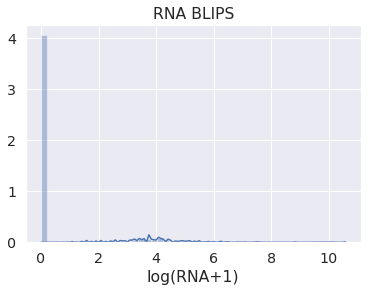
\includegraphics[width=0.45\linewidth]{HIV_distplot_blips}
	}
	\subfloat{
		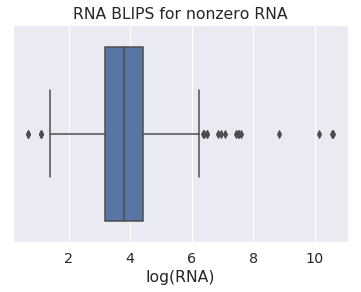
\includegraphics[width=0.45\linewidth]{HIV_histplot_blips_nonzero}
	}
	\caption{Distribution of the viral loads. The Boxplot only includes the non-zero values.}
	
	\label{fig:blipsdist}
\end{figure}
\begin{figure}[h]
	\centering
	\subfloat{
		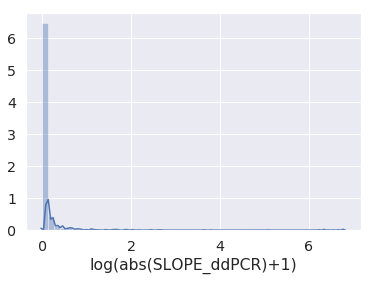
\includegraphics[width=0.48\linewidth]{HIV_distplot_slopelog}
	}
	\subfloat{
		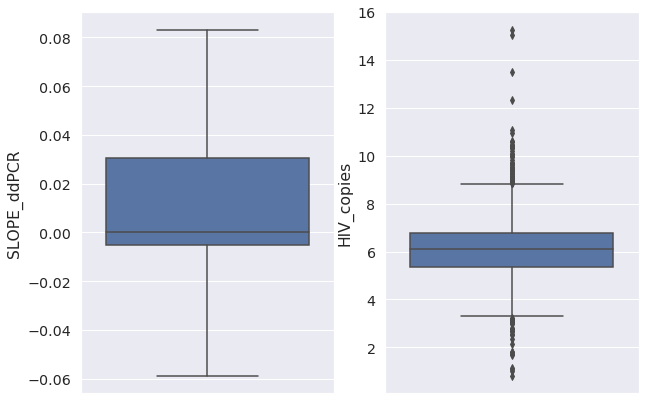
\includegraphics[width=0.48\linewidth]{HIV_histplot_ddPCR}
	}
	\caption{Distribution of ddPCR HIV\_copies and ddPCR slope.}
	
	\label{fig:ddPCRdist}
\end{figure}
In \autoref{fig:ngs_time_diff} the time difference between the NGS and the GRT data is given.
It can be seen that the majority of the GRT mutations are either from the same date as the NGS data (the start of the treatment) or a later point of time (presumably when treatment had to be switched).

The patients in the data set have been observed for up to 14 years (see \autoref{fig:days_since_1stddpcr}), while 
the NGS testing is only done once for each patient.
It would be questionable to assume that the haplotypes of the virus remain unchanged,
over such a long interval and during possibly multiple treatment changes.
For this reason we will only use the first sample of each patient for the network estimation,
as it is closest in time to the NGS data.
\begin{figure}
	\centering
	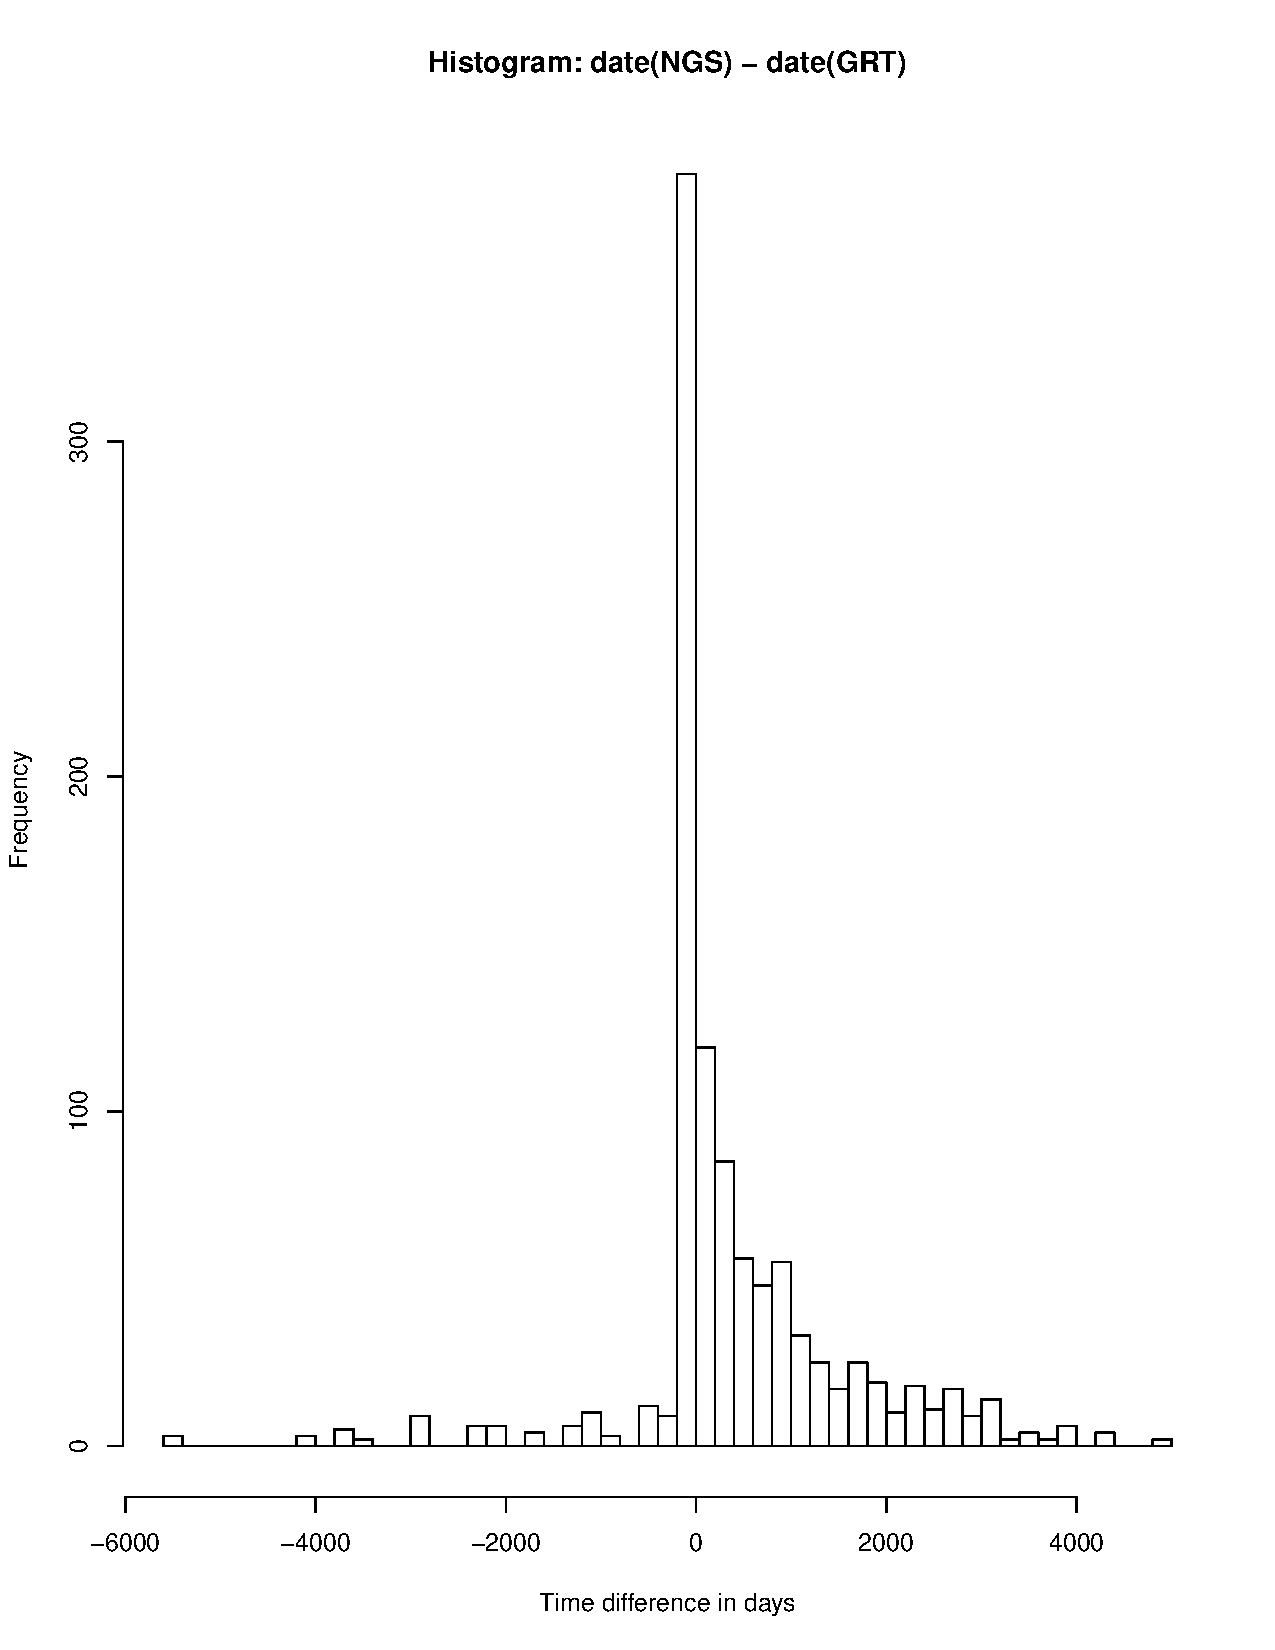
\includegraphics[page=1, width=0.7\textwidth]{NGS_vs_GRT_time}
	\caption{Histogram of patient wise time difference (in days) between the GRT mutations and the NGS data.}
	\label{fig:ngs_time_diff}
\end{figure}
\begin{figure}
	\centering
	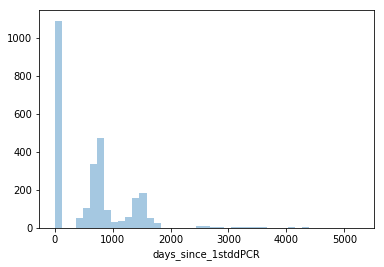
\includegraphics[width=0.6\textwidth]{days_since_1stddpcr}
	\caption{Histogram of time passed between current ddPCR sample and the first ddPCR test of the respective patient.}
	\label{fig:days_since_1stddpcr}
\end{figure}
\FloatBarrier
\ \ \\
\pagebreak
\subsubsection*{Setup}
The settings for the Gibbs BMB and the Annealing run are given in \autoref{table:settings_model_HIV}.
Note that in contrast to the test data setting, no thresholding Credible Interval was set in advance.
\begin{table}[H]
	\centering
	\caption{Model Parameters used for the HIV-X Data\label{table:settings_model_HIV}}
	\begin{tabular}{l c c}
		& \textbf{BMB}   & \textbf{Simulated Annealing} \\
		\toprule
		Total Iterations  & $7000$         & $7000$                       \\\midrule
		Gibbs Sweeps      & $7000$         & $2100$                        \\
		Burn-In           & $2100$          & $630$                        \\
		Cooling Steps     & -              & $4900$                       \\
		Draws at $T_n$    & -              & $490$                        \\
		$T_0$             & -              & $1$                          \\
		$T_n$             & -              & $0.01$                       
	\end{tabular}
\end{table}

% Data description
%% -> source
%% -> haplotype inferred mutations / genotype resistance testing mutations

\subsection{Modality of the Posterior}
Analogous to the test setting, we look at a low dimensional projection of the marginal posterior distribution $ p(\Wxy|\matr{Z}\in D, \lambda)$ 
via PCA.
As it turns out, the $\Wxy$ posterior appears to be multi-modal for $\lambda$ lower than 250,
while being unimodal for higher $\lambda$.
Figures \ref{fig:unimodality_HIV200} and \ref{fig:unimodality_HIV300} show the distributions for a $\lambda$ of 200 and 300 respectively.
It should be noted again that the first two principal components for $\lambda=300$ only explain about $32\%$ of the variance in the data,
so the projection is rather inaccurate.
Therefore the conclusion on unimodality should be taken with caution.
When looking at the MCMC diagnostics, we could not find any indications of convergence problems for $\lambda=200$, $\lambda=300$.
A representative example for the diagnostic plots is shown in \autoref{fig:diagnostics200} and \autoref{fig:diagnostics300}.
Both the autocorrelation and the trace plot seem acceptable.
In contrast, $\lambda$ of 50 and lower are to be avoided, as the autocorrelation indicate repeating fluctuation in the samples (see \autoref{fig:diagnostics50}).

But in general, the multi-modality for low $\lambda$ is not an unexpected observation.
A big part of the HIV data, namely the resistance mutations of the haplotypes and GRT, as well as current and previous treatments, are very sparse.
In addition, there are a lot of missing values for the haplotype mutations and the data is high dimensional ($230$ variables for $1092$ samples).
Therefore it is reasonable that various configurations are capable of explaining the data, if the prior does not enforce a lot of sparsity in the parameters.
As a consequence we will avoid the annealing in this $\lambda$ region.

%%%%%%%%%%%%%% multiple modes HIV data
\begin{figure}[H]
	\centering
	\subfloat{
		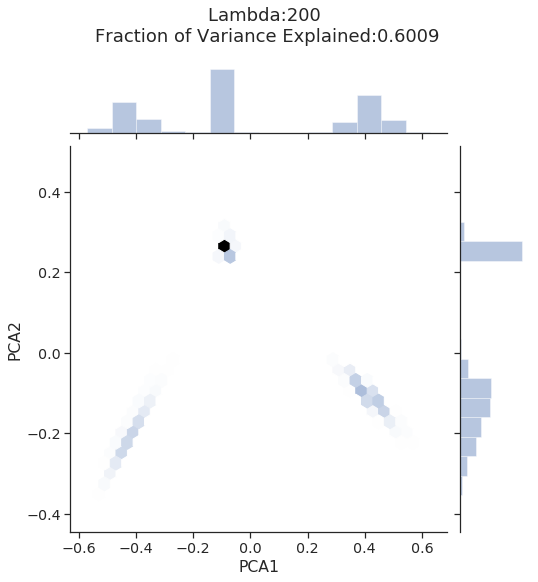
\includegraphics[width=0.48\linewidth]{PCA_W12_HIV_l200}
	}
	\subfloat{
		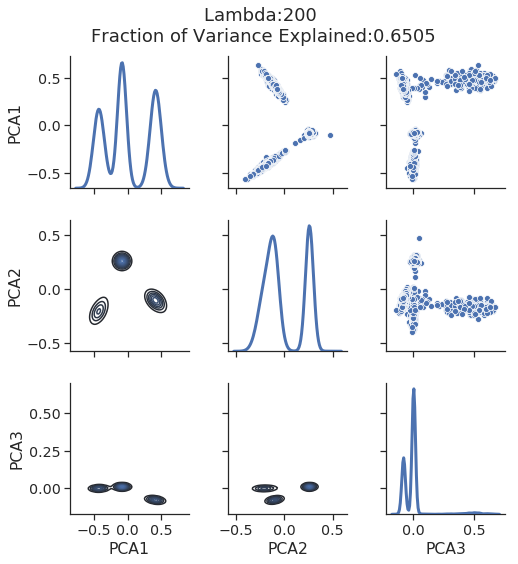
\includegraphics[width=0.48\linewidth]{PCA_W12_HIV_l200_2}
	}
	\caption{Empirical distribution of the $\Wxy$ posterior marginal over the first principal components with $\lambda=200$.}
	
	\label{fig:unimodality_HIV200}
\end{figure}
%%%%%%%%%%%%%%% one mode HIV data
\begin{figure}[H]
	\centering
	\subfloat{
		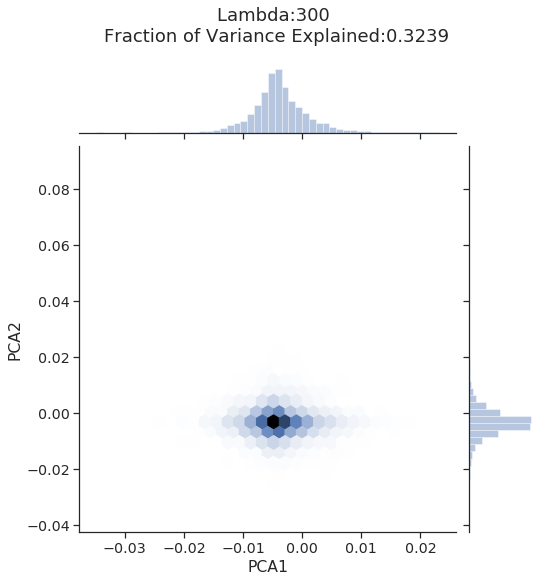
\includegraphics[width=0.48\linewidth]{PCA_W12_HIV_l300}
	}
	\subfloat{
		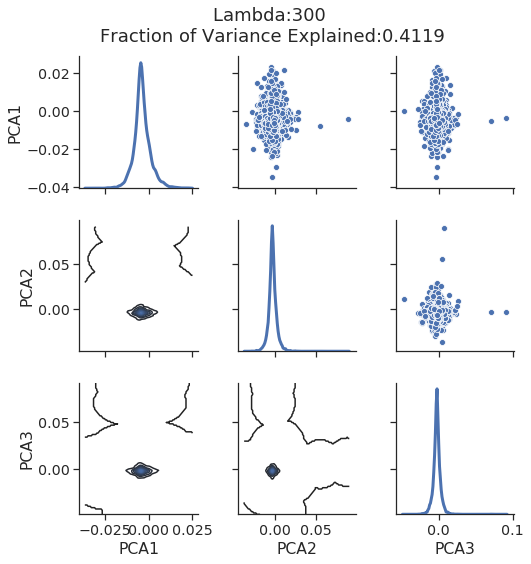
\includegraphics[width=0.48\linewidth]{PCA_W12_HIV_l300_2}
	}
	\caption{Empirical distribution of the $\Wxy$ posterior marginal over the first principal components with $\lambda=300$.}
	
	\label{fig:unimodality_HIV300}
\end{figure}

%%%%%%%%%%%%%% MCMC diagnostics 200 vs 300
\begin{figure}[H]
	\centering
	\subfloat{
		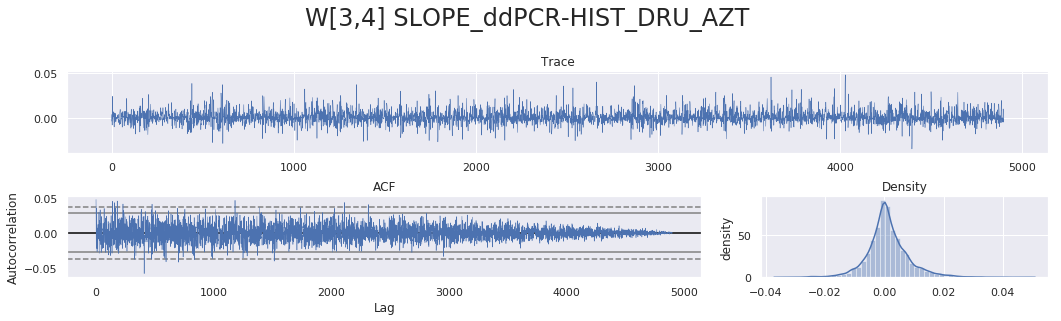
\includegraphics[width=0.9\linewidth]{HIV_MCMC_diag_l200}
		\caption{MCMC diagnostics for the Gibbs sampler with $\lambda=200$. Note that W in this case refers to $W_{12}$.}
		\label{fig:diagnostics200}
	}
	\qquad\qquad\qquad\\
	\qquad\qquad\qquad
	\subfloat{
		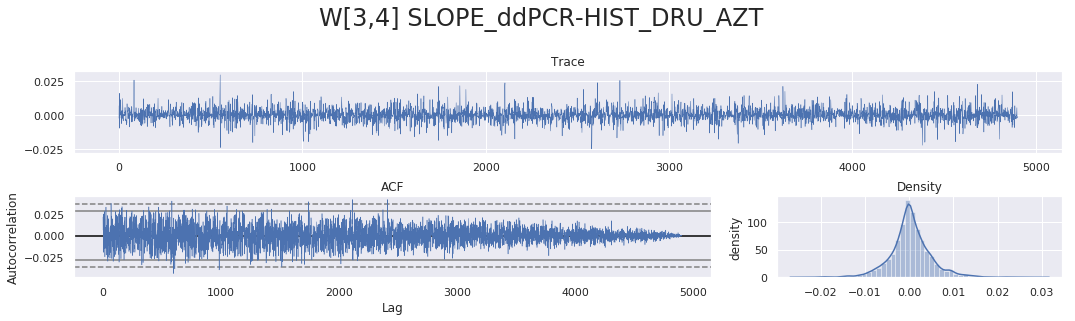
\includegraphics[width=0.9\linewidth]{HIV_MCMC_diag_l300}
		\caption{MCMC diagnostics for the Gibbs sampler with $\lambda=300$. Note that W in this case refers to $W_{12}$.}
		\label{fig:diagnostics300}
	}
	\qquad\qquad\qquad\\
	\qquad\qquad\qquad
	\subfloat{
		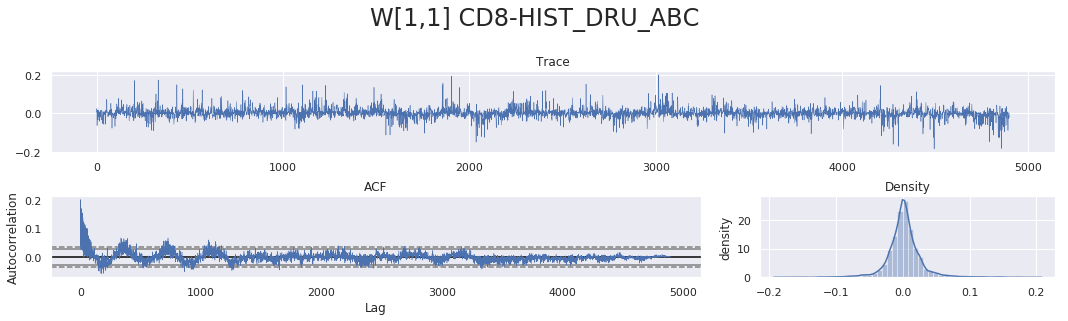
\includegraphics[width=0.9\linewidth]{HIV_MCMC_diag_l50}
		\caption{MCMC diagnostics for the Gibbs sampler with $\lambda=50$. Note that W in this case refers to $W_{12}$.}
		\label{fig:diagnostics50}
	}
\end{figure}




\subsection{Selection of Lambda and Threshold}
First of all, the network sizes for different $\lambda$ and thresholds were explored.
As we can see in \autoref{fig:heatmapSA}, Simulated Annealing leads to a smooth change in network size
over the range of $\lambda$ and thresholds explored, which is what we would expect.
This allows us to fix the thresholding while exploring the whole range of networks, from rather densely connected to completely sparse.
As we know that both precision and specificity tend to increase with network sparsity,
connections found in sparser networks (i.e. with higher $\lambda$) can be seen as more certain.
%%%%%%%%%%% HEATMAP SA
\begin{figure}[H]
	\centering
	\subfloat{
		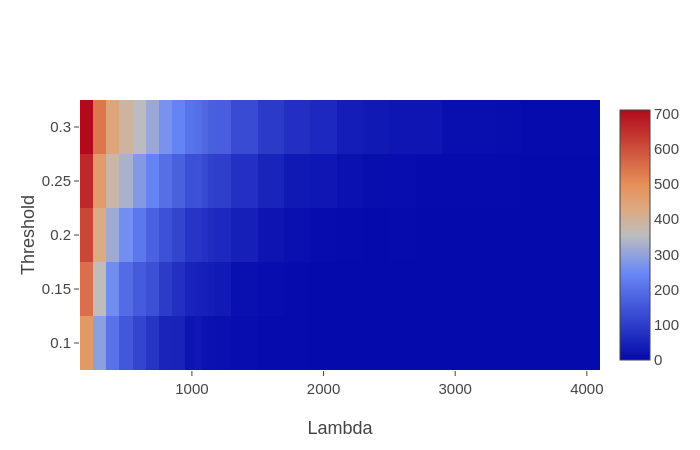
\includegraphics[width=0.48\linewidth]{HIV_SA_heat}
	}
	\subfloat{
		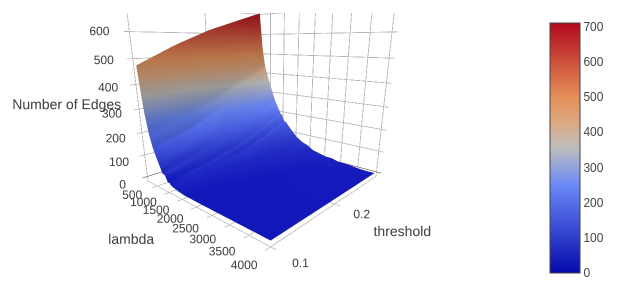
\includegraphics[width=0.48\linewidth]{HIV_SA_heat3d}
	}
	\caption{Heatmap and 3D surface plot showing the number of edges in the inferred networks with the SA BMB for different $\lambda$ and Credible Intervals (\gls{CI} defined by [threshold, 1-threshold]).}
	
	\label{fig:heatmapSA}
\end{figure}


In contrast, finding a suitable range of $\lambda$ for the Gibbs \gls{BMB} is quite difficult.
As shown in \autoref{fig:heatmapgibbs},  the resulting networks are non-trivial for reasonable Credible Intervals only in the multi-modal region $(\lambda<200)$.
But even then, the resulting networks are extremely sparse for 80\% Credible Intervals and above,
with a non-smooth and non-monotonic decrease in the number of edges for higher $\lambda$.
As with SA, we know the precision and specificity generally increases for higher $\lambda$ and sparser networks.
However, the usable range of $\lambda$ is very close to the range subject to convergence problems.
While we can clearly see that $\lambda$ of 50 and lower are unusable, it is not certain that slightly higher $\lambda$
are immune; it is possible, that similar problems are not obvious from mere inspection of the diagnostic plots.
Combined with non-monotonic change of network size, network and model exploration is made considerably more difficult.
%%%%%%%%%% HEATMAP gibbs
\begin{figure}[H]
	\centering
	\subfloat{
		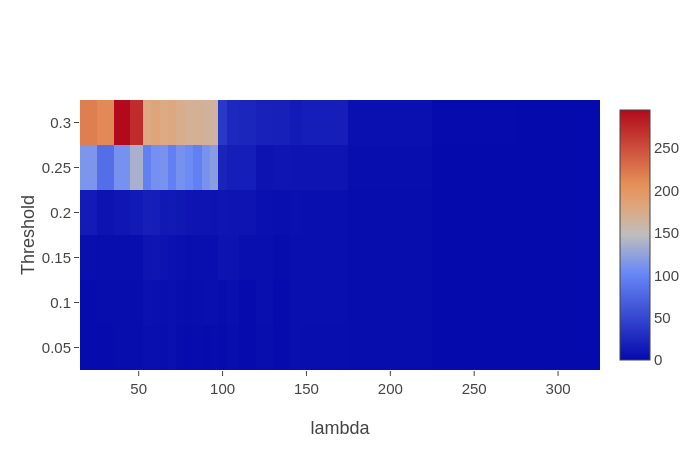
\includegraphics[width=0.48\linewidth]{HIV_gibbs_heat}
	}
	\subfloat{
		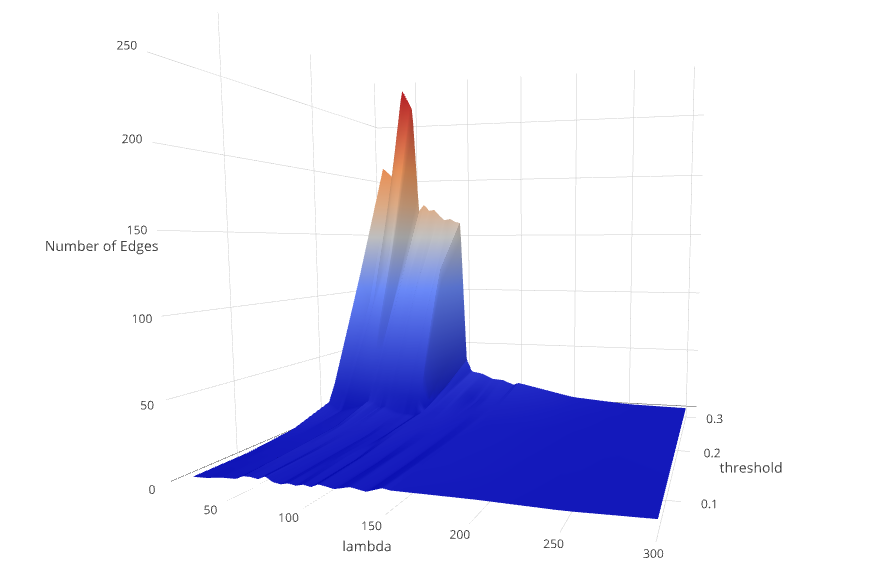
\includegraphics[width=0.48\linewidth]{HIV_gibbs_heat3d}
	}
	\caption{Heatmap and 3D surface plot showing the number of edges in the inferred networks with the Gibbs BMB for different $\lambda$ and Credible Intervals (\gls{CI} defined by [threshold, 1-threshold]).}
	
	\label{fig:heatmapgibbs}
\end{figure}
\pagebreak

\subsection{Dependencies by Relevance}
Starting from the sparsest graph we can decrease the $\lambda$ in small steps and look at which edges are added.
It is important to note, that edges can in some cases vanish again for smaller $\lambda$.
That is, the network resulting from a higher $\lambda$ are not always subsets of the denser networks.
It is unclear, whether this is occurs due to convergence issues of the Annealing or simply is part of the models behavior.
Nonetheless, the increase in specificity and precision for higher $\lambda$ is still relevant.
\autoref{fig:HIVbylambda1} shows edges that have been observed for a $\lambda$ of 1400 and higher with a threshold of $0.15$.
The plotted bars correspond to the highest $\lambda$ they were observed at, i.e. the sparsest network that still contained them.

\begin{figure}
	\centering
	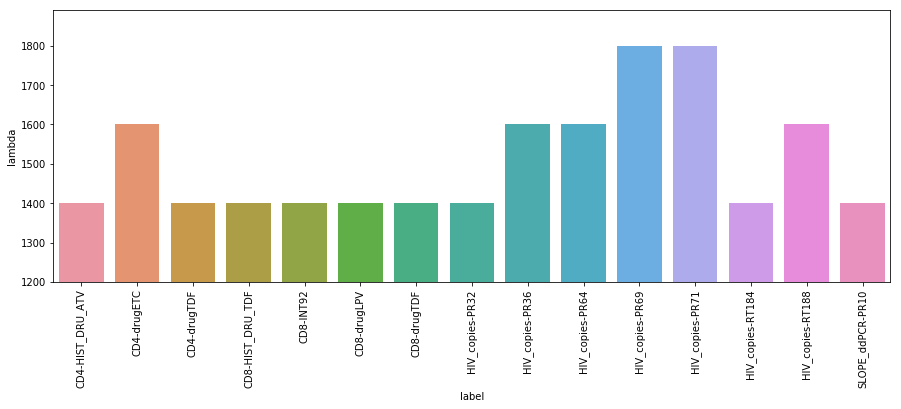
\includegraphics[width=1\linewidth]{HIV_bylambda}
	\caption{Maximum $\lambda$ for which each edge was observed with threshold $0.15$ and $\lambda>=1400$.}
	\label{fig:HIVbylambda1}
	
\end{figure}
We can see that about half of the dependencies there correspond to connections between the ddPCR counts (or its slope) and resistance relevant mutations from the haplotypes.
The two first edges correspond to the haplotype mutations PR69 and PR71.
According to \cite{shafer2017human}, PR69 is associated only with the \gls{PI} tipranavir,
which has shown to be effective for patients being resistant to other PIs \citep{doyon2005selection}.
Thus a mutation restricting the effectiveness of tipranavir being relevant for the HIV levels of treatment experienced patients seems reasonable.
PR71 is associated with multi-drug resistance for five different \gls{PI}s (of totally 8).
Considering that, this resistance can limit the range of possible \gls{PI} in a treatment considerably, making it an important factor for successful \gls{ART}.
In general we can see that a large portion of the first few dependencies correspond to resistances against protease inhibitors.
For the interested reader \autoref{fig:HIVbylambda2} additionally provides the edges found for $\lambda$ greater than 1000 and smaller than 1400.
We will not go into further details at this point and instead switch to the network graphs.
\begin{figure}[H]
	\centering
	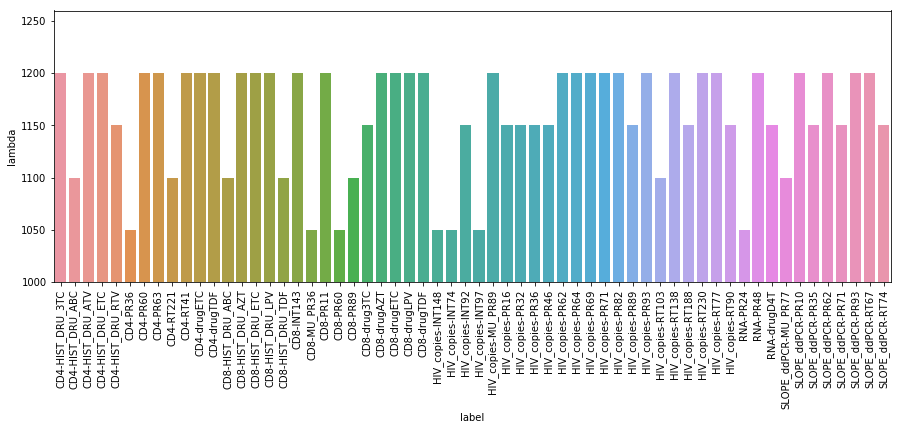
\includegraphics[width=1\linewidth]{HIV_bylambda_1000p}
	\caption{Maximum $\lambda$ for which each edge was observed with threshold $0.15$ and $1000<\lambda<1400$.}
	\label{fig:HIVbylambda2}
	
\end{figure}
\subsection{Dependency Networks}
For comparing the networks resulting from the BMB and SA, we fix the graph size to 42 non-zero edges and then select a corresponding threshold and $\lambda$, which leads in our opinion to a network size that is still interpretable while not being trivial.
In case of the Annealing, we left the threshold fixed at $0.15$ with a $\lambda$ of 1100.
For the BMB, the threshold had to be finely tuned, resulting in a $\lambda$ of 70 with the threshold $0.22$.
In \autoref{fig:bignetworkcircle} and \autoref{fig:bignetworkcircle2} the network graphs are shown in a circular layout.
It can be seen, that the networks resulting from the BMB and the SA are rather similar.
Both exhibit a lot of connections with the lower section of the circle, which corresponds to the mutations calculated from the reconstructed haplotypes.
In contrast, there are barely any connections to the left side, i.e. the GRT mutations.
Simulated Annealing finds one dependency there, while the BMB does not show any.
The found edge corresponds to a positive partial correlation between MU\_PR77 affecting 3 different \gls{PI}s and the ddPCR slope, indicating a deterioration caused by the mutation.
However, it is unclear why barely any interactions with the GRT mutations are present in the networks.
Examining GRT mutations for planning the next step in a antiretroviral therapy is currently a standard practice, due to the shown improvements in terms of therapy success \cite{gunthard2018human}.
Instead of assuming a lack of dependency between the clinical factors and the GRT mutations, this might indicate that the mutations inferred from the haplotypes are more accurate,
thus making the GRT mutations mostly redundant when conditioning on the haplotypes.

%%%%%%%% BIG NETWORK CIRCLE
\begin{figure}
	\centering
	\includegraphics[width=0.72\linewidth]{HIV_gibbs_bigcircle}
	
	\caption{W12 subnetwork estimated with Gibbs BMB.}
	\label{fig:bignetworkcircle}
\end{figure}
\begin{figure}
	\centering
	\subfloat{
		\includegraphics[width=0.72\linewidth]{HIV_SA_bigcircle}
		\caption{W12 subnetwork estimated with SA.}
		\label{fig:bignetworkcircle2}
	}
	
\end{figure}
\autoref{fig:network_gibbs} and \autoref{fig:network_SA} show the the same networks with a different layout.
Here we can see that a lot of haplotype mutations form a cluster around the ddPCR values (in case of the SA also around the slope).
While the connections themselves seem reasonable, the signs of the partial correlations are counter-intuitive.
A red edge corresponds to a negative partial correlation.
Consequently, a lot of haplotype mutations would seem to result in a decrease of the HIV levels.
Instead, we would have expected an increase, as the resistance relevant mutations generally inhibit the effectiveness of specific drugs.
Furthermore, we can see that ETC and TDF have a positive edge to the CD4 values, while simultaneously being negatively correlated with the CD8 counts. 
In the initial phase of HIV infection, the CD8 counts increase significantly and are followed by a decrease of CD4 counts.
In addition the ratio of CD4 to CD8 counts is known to be a marker for the clinical outcome in virologically suppressed HIV patients \citep{lu2015cd4} and elevated CD8 counts during ART are associated with failure in antiretroviral therapy \citep{krantz2011elevated}.
As a consequence, we can assume that the positive correlation with CD4 and negative correlation with CD8 counts corresponds to the ETC and TDF having a positive impact on treatment success.

An interesting connection that is present in both networks (see \autoref{fig:intersection}) is the positive partial correlation between RNA and the drug \gls{D4T},
with the Gibbs BMB also showing an edge to HIST\_D4T.
\gls{D4T} is a \gls{NRTI}, meaning that it blocks the enzyme responsible for changing RNA into the form of DNA.
While being largely used in the past as a initial treatment for patients with advanced immunodeficiency \footnote{\href{http://www.aidsmap.com/d4T-stavudine-iZeriti/page/1730937/}{http://www.aidsmap.com/d4T-stavudine-iZeriti/page/1730937/}}
the \gls{WHO} no longer recommends its use due to side effects
 \footnote{
 	\href{http://www.who.int/hiv/pub/guidelines/arv2013/arv2013supplement_to_chapter09.pdf}
	{http://www.who.int/hiv/pub/guidelines/arv2013/arv2013supplement\_to\_chapter09.pdf}}.
The connection might indicate that patients starting treatment at a later stage show a higher tendency for exhibiting blips in therapy.
In any case, the connections between viral load and \gls{ART} drugs do not shed any light on the controversial effects of the blips on developing new resistance mutations.


%% -> Networks: BMB + SA
\begin{figure}
	\centering
	\makebox[\textwidth][c]{
		\includegraphics[width=1.2\linewidth]{HIV_gibbs_network}
	}
	\caption{Inferred network with Gibbs BMB, using $\lambda$ = 70 and threshold $0.22$.}
	\label{fig:network_gibbs}
\end{figure}
\begin{figure}
	\centering
	\makebox[\textwidth][c]{
		\includegraphics[width=1.2\linewidth]{HIV_SA_network}
	}
	
	\caption{Inferred network with Simulated Annealing, using $\lambda$ = 1100 and threshold $0.15$.}
	
	\label{fig:network_SA}
\end{figure}
\begin{figure}
	\centering
	\includegraphics[width=0.9\linewidth]{HIV_intersection_network}
	\caption{Intersection of the SA and BMB network. Black edges indicate a disagreement in the sign of the edge.}
	
	\label{fig:intersection}
\end{figure}

\FloatBarrier
\subsection{Latent Scores}
\autoref{fig:zscores} and \autoref{fig:zscores_bool} illustrate the effect of the copula transformation on the data
for 2100 Gibbs sweeps with a burn-in of 630 and a $\lambda$ of 1000.
The first column shows the distribution of untransformed observations for one variable;
the second, the distribution of the normal scores (which are used for initialization);
the third column shows the distribution of the posterior mean of the latent values.
That is, the histogram of the estimated $E[z_{i,j}|\matr{Z}\in D, \lambda=1000]$ for all observations $i$ with fixed variable $j$.
The distributions did not show any significant change with further iteration of the sampler.
The latent values of the remaining query variables are not displayed for the sake of compactness, since they did not show 
any unusual behavior.

\begin{figure}[H]
	\centering
	
	\subfloat{
		\includegraphics[width=0.9\linewidth]{HIV_Zscores_RNA}
	}
	\subfloat{
		\includegraphics[width=0.9\linewidth]{HIV_Zscores_ddpcr}
	}
	\caption{Initial distribution of the data compared to the distribution of the estimated latent values.}
	\label{fig:zscores}
\end{figure}
The semi-parametric copula seems to be troubled mainly when the data is highly imbalanced with a lot of identical values.
While the estimated latent values for the ddPCR count and even the boolean HIST\_DRU\_3TC are relatively normal,
the viral load (RNA) and the GRT mutations (in this case MU\_RT70) seem to be flawed.
The RNA is similar to the GRT mutations in the sense that it has the majority of samples at the same value $0$,
with the exception of a few blips.
In contrast, the variables indicating the per-drug treatment-experience are more balanced.
Additionally, the mutations inferred from the haplotypes contain a lot of missing values, which are filled by the copula sampler
with normal draws.
That the unbalanced GRT mutations do seemingly not converge to a normal distribution might be related to the failure to find dependencies shared with the query variables.

\begin{figure}
	\subfloat{
		\includegraphics[width=0.9\linewidth]{HIV_Zscores_HIST3tc}
	}
	\subfloat{
		\includegraphics[width=0.9\linewidth]{HIV_Zscores_PR13}
	}
	\subfloat{
		\includegraphics[width=0.9\linewidth]{HIV_Zscores_MU_RT70}
	}
	\caption{Initial distribution of the data compared to Z estimated by averaging over the draws. The second column corresponds to the distribution of the normal scores, the last column to the mean over all draws.}
	\label{fig:zscores_bool}
\end{figure}
%% -> Latent Variables: Not fully normal
%% -> Talk about connections found